\documentclass[article,11pt, reqno]{article}
\usepackage{amsfonts, amsmath, amssymb, amsthm, mathtools, mathrsfs, geometry, dsfont, tikz-cd, verbatim}
\usepackage{hyperref}[hidelinks]
\usepackage[T2A]{fontenc}
\usepackage{hyphenat}
%\usepackage[dvipsnames]{xcolor}
\hyphenation{ма-те-ма-ти-ка вос-ста-нав-ли-вать}
%\usepackage[english, russian]{babel}
\hypersetup{
    colorlinks,
    citecolor=black,
    filecolor=black,
    linkcolor=black,
    urlcolor=black
}
\geometry{letterpaper, margin=0.7in}

\usepackage{setspace}
\setstretch{1.25}

\usepackage{blindtext}
%\usepackage[hidelinks]{hyperref}
\usepackage[explicit]{titlesec}
\titleformat{\section}
{\normalfont\Large\bfseries}{\thesection}{1em}{\hyperlink{sec-\thesection}{#1}
\addtocontents{toc}{\protect\hypertarget{sec-\thesection}{}}}
\titleformat{name=\section,numberless}
{\normalfont\Large\bfseries}{}{0pt}{#1}

\newtheorem*{theorem}{Theorem}
\newtheorem*{corollary}{Corollary}
\newtheorem*{lemma}{Lemma}
\newtheorem*{proposition}{Proposition}
\newtheorem*{definition}{Definition}

\theoremstyle{remark}
\newtheorem*{remark}{Remark}
\newtheorem*{example}{Example}
\newtheorem*{note}{Note}
\newtheorem*{claim}{Claim}
\newtheorem*{notation}{Notation}

\renewcommand{\baselinestretch}{1}

\newcommand{\tb}{\textbf}
\newcommand{\R}{\mathbb{R}}
\newcommand{\N}{\mathbb{N}}
\newcommand{\Ra}{\Rightarrow}
\newcommand{\La}{\Leftarrow}
\newcommand{\inv}{^{-1}}
\newcommand{\wt}{\widetilde}
\newcommand{\wh}{\widehat}
\newcommand{\mb}{\mathbb}
\newcommand{\mc}{\mathcal}
\DeclareMathOperator{\interior}{Int}
\DeclareMathOperator{\id}{id}

\newcommand{\tl}{\triangleleft}
\newcommand{\ra}{\rightarrow}
\newcommand{\Q}{\mathbb{Q}}
\newcommand{\F}{\mathbb{F}}
\newcommand{\pN}{\wp(\mathbb{N})}
\newcommand{\Z}{\mathbb{Z}}
\newcommand{\cc}{\mathbf{c}}
\newcommand{\ec}[1]{\overline{#1}}
\newcommand{\lub}{\text{lub}}
\newcommand{\MAX}{\text{Max}}
\newcommand{\glb}{\text{glb}}
\newcommand{\MIN}{\text{Min}}
\newcommand{\I}{\mathcal{I}}
\newcommand{\rk}{\text{rk}}
\newcommand{\ups}{{}^\sharp}
\newcommand{\K}{\mathbb{K}}
\newcommand{\<}{\langle}
\renewcommand{\>}{\rangle}
\newcommand{\e}{\epsilon}
\newcommand{\ex}{\exists}
\newcommand{\pf}{\textit{Proof: }}
\newcommand{\gal}{\text{Gal}}
\newcommand{\aut}{\text{Aut}}
\newcommand{\im}{\text{im}}
\newcommand*\circled[1]{\tikz[baseline=(char.base)]{
            \node[shape=circle,draw,inner sep=0.5pt] (char) {#1};}}
\title{\textbf{\textsc{Ма 535 Конспект Лекций}}}
\author{\textsc{Fung San Gaan and Jihong Cai}}
\date{Fall 2023}

\begin{document}
\maketitle
\tableofcontents
\section{Metric Space}
\subsection*{Euclidean Distance}
Recall the standard Euclidean metric on $\mb R^2$. The \tb{Euclidean distance} $d_{Euc}:\mb R^2\times \mb R^2\rightarrow [0,\infty)$ is a function defined as
$$d_{Euc}(x,y):=\sqrt{(x_1-y_1)^2+(x_2-y_2)^2}.$$

We can generalize this function to $\mb R^n$ where $n<\infty$ by $d_{Euc}:\mb R^n\times \mb R^n\rightarrow [0,\infty)$ where
$$d_{Euc}(x,y):=(\sum_1^n (x_i-y_i)^2)^{1/2}.$$

There are three important properties of the Euclidean distance that we would like to extract for a more abstract notion of distance.

\subsection*{Metric Spaces}
A \tb{metric} is a distance measuring function $d: X\times X\rightarrow [0,\infty)$ satisfying
\begin{enumerate}
    \item Nondegeneracy. $d(x,y)=0$ if and only if $x=y$ for all $x,y\in X$.
    \item Symmetry. $d(x,y)=d(y,x)$ for all $x,y\in X$.
    \item Triangular Inequality. $d(x,z)\leq d(x,y)+d(y,z)$ for all $x,y, z\in X$.
\end{enumerate}
A pair $(X,d)$, where $X$ is a set and $d:X\times X\rightarrow [0,\infty)$ is a metric, is called a \tb{metric space}.

\begin{example}
    $(\mb R^n, d_{Euc})$ is a metric space.
\end{example}
\begin{example}
    A vector space with inner product $(V, \langle\cdot,\cdot\rangle)$ is a metric space.
\end{example}

The set $B(x_0,r)$ is called an \tb{open ball in $X$} at center $x_0$ with radius $r$ if
$$B(x_0,r):=\{y\in X\ |\ d(y, x_0)<1\}$$
with respect to some metric $d$.

An open set in $X$ is a union of open balls in $X$. That is, $U$ is open in $X$ if 
$$U=\bigcup_{\alpha\in I} B(x_{0_\alpha},r_\alpha).$$
\begin{example}
    Open balls in $\mb R$ are open intervals. Open sets in $\mb R$ are disjoint unions of open intervals.
\end{example}
\noindent
\fbox{\begin{minipage}{47em}
            \begin{proposition}[1.2.1]
    Open ball $B(x_0,r)$ is open in $X$.
\end{proposition}
        \end{minipage}}
\begin{proof}
    Take any point $y\in B(x_0,r)$. We need to show that there exists $B(y,\rho)\subseteq B(x_0,r)$ for some $\rho>0$. Take $\rho=\frac{r-d(x_0,y)}{2}$, and $B(y,\rho)\subseteq B(x_0,r)$. (Take a smaller ball!)
\end{proof}

Consider the boundary of the unit open ball centered at the origin of dimension $n+1$. 
The set $S^n$ is the collection of points such that 
$$S^n:=\{y\in\mb R^{n+1}\ | \ d(y, 0)=1\}$$
is called \tb{sphere of dimension $n$}.

We can now take the closure of the unit open ball centered at the origin.
The set $D^n$ is called \tb{disc of dimension $n$} if
$$D^n:=\{y\in\mb R^{n}\ | \ d(y, 0)=1\}.$$


\section{Definition of Topological Spaces}
\subsection*{Motivation and Construction of Topological Spaces on $\mb R^n$}
\begin{notation}
    For $\mc F$ a collection of subsets in $X$. Denote
    $$\bigcup\mc F:=\bigcup_{U\in\mc F} U:=\{y\in X\ |\ \text{there exists } U\in\mc F \text{ such that } y\in U\}$$
    and
    $$\bigcap\mc F:=\bigcap_{U\in\mc F} U:=\{y\in X\ |\ \text{for all } U\in\mc F, y\in U\}.$$
\end{notation}

Suppose $\mc B$ denotes the collections of all open balls in $\mb R^n$. That is, 
$$\mc B:= \{B(x,r)\ | \ x\in\mb R^n, r\in[0,\infty)\}.$$ Let $\mc B'$ be any subcollection of $\mc B$, i.e. $\mc B'\subseteq\mc B$. Let 
$$\mc T=\bigcup \mc B'=\{\bigcup_{B\in\mc B'} B\ | \ \mc B'\subseteq \mc B\}.$$ The following two properties hold:
Given $U_1, U_2\in\mc T$ where $U_1=\bigcup_{U\in \mc B_1} U$ and $U_2=\bigcup_{U\in \mc B_2} U$, 
\begin{enumerate}
    \item $U_1\cup U_2\in\mc T$, because $U_1\cup U_2=(\bigcup_{U\in \mc B_1} U)\cup (\bigcup_{U\in \mc B_2} U) = \bigcup_{U\in \mc B_1\cup B_2} U$. In fact, it is true that $\bigcup_{i\in I} U_i$ for an arbitrarily large index set.
    \item $U_1\cap U_2\in\mc T$, because $U_1\cap U_2=(\bigcup_{U\in \mc B_1} U)\cap (\bigcup_{U'\in \mc B_2} U') = \bigcup_{U\in\mc B_1, U'\in\mc B_2} (U\cap U')\in\mc T$
\end{enumerate}

\subsection*{Topological Spaces}
We will take these properties into a definition.
A \tb{topology} on $X$ is a collection of subsets $\mc T\subseteq \mc P(X)$ such that
\begin{enumerate}
    \item $\varnothing, X\in\mc T$,
    \item given $\{U_i\}_{i\in I}, \bigcup_{i\in I} U_i\in\mc T$, and
    \item given $U_1, U_2\in\mc T$, $U_1\cap U_2\in T$.
\end{enumerate}
That means a topology is closed under arbitrary union and finite intersection. A pair $(X, \mc T)$, where $X$ is a universal set and $\mc T$ is some topology on it is called \tb{topological space}.
\begin{example}
    The collection $\mc T=\{\varnothing, X\}$ is a topology. It is, in fact, the smallest topology of a given set $X$, usually called trivial topology or indiscrete topology.
\end{example}
\begin{example}
    The collection $\mc T=\mc P(X)$ is a topology. This is the largest topology on $X$ called discrete topology.
\end{example}
\begin{example}
    In $\mb R^n$, the union of open balls is called open sets. The collection of such open sets in $\mb R^n$ forms a topology.
\end{example}

Elements in a topology are called \tb{open sets}, and their complements are called \tb{closed sets}. I.e., if $U$ is open in $X$, $U^c=X\backslash U$ is closed.

Note that open sets are not closed under arbitrary intersections. For example, verify that 
$$\bigcup_1^\infty (-\frac{1}{n}, 1+\frac{1}{n}) = [0,1]$$
and $[0,1]$ is not open in $\mb R$.
Similarly, closed sets are not closed under arbitrary union. For example, $$\bigcup_1^\infty [\frac{1}{n}, 1-\frac{1}{n}]=(0,1)$$.\\
\fbox{\begin{minipage}{47em}
            \begin{lemma}[2.2.1]
    Let $X$ be a set and $\mc T$ be a topology on $X$. Let $\mc T'$ be a family of all closed subsets of $X$, then $\mc T'$ satisfies
    \begin{enumerate}
        \item $\varnothing, X\in\mc T'$
        \item $\mc T'$ is closed under arbitrary intersections
        \item $\mc T'$ is closed under finite union.
    \end{enumerate}
\end{lemma}
        \end{minipage}}
\begin{proof}
\begin{enumerate}
    \item  $\varnothing$ is closed by definition. This is a vacuously true statement.
    $X$ is the complement of $\varnothing$. Because $\varnothing$ is open, $X$ is closed.
    \item Let $\{C_i\}_{i\in I}$ be a family of closed subsets of $X$, $X\backslash (\bigcap_{i\in I} C_i) = \bigcup_{i\in I} (X\backslash C_i)\in\mc T$.
    \item Let $C_1, C_2\in\mc T'$ be two closed sets in $X$, 
    $X\backslash (C_1\cup C_2) = (X\backslash C_1)\cap (X\backslash C_2)\in \mc T$.
\end{enumerate}
   
\end{proof}

Hence, any topology can be equivalently described using closed sets.


A \tb{neighborhood} of $x\in X$ is an open set $U\subseteq X$ containing $x$.


Any topology induced by a metric space $X$ is called a \tb{metric topology}. We will talk about metric topology in depth later in the course.

A topological space $(X,\mc T)$ is called \tb{Hausdorff} if for all $x,y\in X$ and $x\neq y$, there exists open sets $U_1$ and $U_2$ in $\mc T$ such that $x\in U_1$, $y\in U_2$, and $U_1\cap U_2=\varnothing$.


\section{Basis and Subbasis}
\subsection*{Basis}
Topological spaces are usually humongous. It is usually impossible to list all the open sets in a topological space. Hence, we want some ways we can construct topological spaces. One of which is via the basis of a topology.

Given a universal set $X$. A \tb{basis} of a topology on $X$ is a collection of subsets $\mc B\subseteq\mc P(X)$ in $X$ such that
\begin{enumerate}
    \item for all $x\in X$, there exists $B\in\mc B$ such that $x\in B$ (equivalently, $\mc B$ covers $X$, i.e. $\bigcup\mc B = X$).
    \item for all $B_1, B_2\in\mc B$, for all $x\in B_1\cap B_2$, there exists $B_3\in\mc B$ such that $x\in B_3\subseteq B_1\cap B_2$
\end{enumerate}
Let $\mc B$ be a basis of a topology. The \tb{topology generated by $\mc B$} is defined as all possible unions of elements in $\mc B$, i.e. 
$$\mc T(\mc B):=\{\bigcup \mc B'\ | \ \mc B'\subseteq\mc B\}.$$
If $\mc B$ satisfies these two conditions, then we define \textbf{the topology $\mc T$ generated by} $\mc B$ as follows: A subset $U$ of $X$ is said to be open in $X$ (that is, to be an element of $\mc T$) if for each $x\in U$, there is a basis element $B \in \mc B$ such that $x\in B$ and $B \subset U$. Note that each basis element is itself an element of $\mc T$.\\
\fbox{\begin{minipage}{47em}
            \begin{lemma}[3.1.1]
    If $\mc B$ is a basis of a topology on $X$, then $\mc T(\mc B)$ is a topology on $X$.
\end{lemma}
        \end{minipage}}
\begin{proof}
    $\varnothing\in \mc T(\mc B)$ because $\varnothing = \bigcup\varnothing\in \mc T(\mc B)$. $X\in \mc T(\mc B)$ because for all $x\in X$, choose $B_x\in \mc B$ such that $x\in B_x$. Then $X=\bigcup B_x\in \mc T(\mc B)$.

    Let $\{U_i\}_{i\in I}$ be a family of elements in $\mc T(\mc B)$. We can write each $U_i$ as a union of subsets in $\mc B$, call it $\mc B_i\subseteq \mc B$. Now $\bigcup U_i= \bigcup_{i\in I} \bigcup B_i$. Because $\mc T(\mc B)$ is a topology, it is closed under arbitrary union. Hence $\bigcup_{i\in I} U_i\in\mc T(\mc B)$.

    Take $U_1, U_2\in \mc T(\mc B)$, $U_1 = \bigcup \mc B_1$ and $U_2 = \bigcup \mc B_2$. Then $U_1\cap U_2 = (\bigcup\mc B_1)\cap(\bigcup \mc B_2) = \bigcup_{U_1\in\mc B_1, U_2\in\mc B_2} (U_1\cap U_2)$. By (2), we know that for all points in $U_1\cap U_2$, there exists $B_3\subseteq B_1\cap B_2$. $\forall x\in B_3$, $B_3\subset U_1\cap U_2$. This shows $U_1\cap U_2\in\mc T$ by the second definition.
\end{proof}


Suppose $\mc T$ is a topology on $X$. $\mc B$ is a collection of subset in $X$ such that is it a basis. We say $\mc B$ is a basis for $\mc T$ if
\begin{enumerate}
    \item $\mc B$ is a basis of some topology and
    \item $\mc T=\mc T(\mc B)$.
\end{enumerate}
\begin{example}
    The topology is a basis of itself.
\end{example}
\begin{example}
    The collection of open balls forms a basis for standard topology on $\mb R^n$.
\end{example}
\begin{example}
    The collection of all singletons forms a basis for discrete topology.
\end{example}


\subsection*{Comparing Topologies}
We say that a topology $\mc T$ is \tb{stronger, larger, or finer} than $\mc T'$ if $\mc T'\subseteq\mc T$. Conversely, we say $\mc T$ is \tb{smaller, coarser, or weaker} than $\mc T'$ is $\mc T\subseteq\mc T'$. The trivial topology is the smallest topology on $X$ and the discrete topology is the largest one on $X$.\\
\fbox{\begin{minipage}{47em}
            \begin{lemma}[3.2.1]
    Suppose $\mc B$ and $\mc B'$ are basis for some topology, then $\mc T(\mc B')$ is larger (stronger) then $\mc T(\mc B)$ if and only if for all $x\in X$, and for all $x\in B\in \mc B$, there exists $B'\in\mc B'$ such that $x\in B'\subseteq B$.
\end{lemma}
        \end{minipage}}
\begin{proof}
    We are given $x \in X$ and $B\in\mc B$, with $x \in B$. Now $B$ belongs to $\mc T$ by definition and $\mc T \subset \mc T'$ by assumption; therefore, $B \in \mc T'$. Notice this means $B$ is open in $\mc T'$. Since $\mc T'$ is generated by $\mc B'$, there is an element $B'\in\mc B'$ such that $x \in B'\subset B$.

    Given an element $U$ of $\mc T$, let $x\in U$. Since $\mc B$ generates $\mc T$, there is an element $B\in\mc B$ such that $x\in B \subset U$. By assumption, there exists an element $B' \in \mc B'$ such that $x\in B'\subset B\subset U$. Then $x \in B' \subset U$, so $U\in \mc T'$, by definition. Since $U$ is an arbitrary set, the converse is proven.
\end{proof}
\noindent
\fbox{\begin{minipage}{47em}
            \begin{lemma}[3.2.2]
    Let $(X, \mc T)$ be a topological space and $\mc C\subseteq \mc T$. $\mc C$ is a basis of $\mc T$ if and only if for all $U\in\mc T$ and for all $x\in U$, there exists $C\in\mc C$ such that $x\in C\subseteq U$.
\end{lemma}
        \end{minipage}}
\begin{proof}
    The forward direction is clear by the definition of basis. To show the converse, we need to first show that it is a basis, and a basis for the topology $\mc T$. Take any $x\in X\in\mc T$, there exists $C\in\mc C$ such that $x\in C\subseteq U$. Take $C_1, C_2\in \mc C\subseteq\mc T$ and $x\in C_1\cap C_2$, we know that $x\in C_1\cap C_2\in\mc T$. Then apply the condition to $U=C_1\cap C_2$, then there exists $C\in\mc C$ such that $x\in C\subseteq C_1\cap C_2$. To show that $\mc T=\mc T(\mc C)$, we need to show two-sided inclusion. Because $\mc C\subseteq \mc T$, it is clear that $\mc T(\mc C)\subseteq \mc T$. To show the opposite, take any set $U\in\mc T$, by the condition, we know that there exists $C\in\mc C$ such that $x\in C$ for all $x\in U$. Hence, $U\in\mc T(\mc C)$ for all $U\in\mc T$. That gives $\mc T\subseteq\mc T(\mc C)$.
\end{proof}

\subsection*{Subbasis}
Basis might be too strong in some cases. It requires a subset in every possible intersection. Some collections might not satisfy such property. Hence, we want to define something called a subbasis. A \tb{subbasis} $\mc S$ of a topology in $X$ is a collection of subsets in $X$ such that $\bigcup \mc S=X$. This is the equivalent of saying for all $x\in X$, there exists $S\in\mc S$ such that $x\in S$.

We can generate a basis from a subbasis $\mc S$ in $X$. The \textbf{topology generated by the subbasis} $\mc S$ is defined to be the collection $\mc T$ of all unions of finite intersections of elements of $\mc S$. Define
$$\mc B(\mc S):=\{\bigcap \mc S'\ | \ \mc S' \text{ is a finite subfamily of } \mc S\}.$$
\fbox{\begin{minipage}{47em}
            \begin{lemma}[3.3.1]
    For any subbasis $\mc S$ in $X$, $\mc B(\mc S)$ is a basis of some topology in $X$.
\end{lemma}
        \end{minipage}}
\begin{proof}
%    Because $\mc S\subseteq\mc B(\mc S)$, $X=\bigcup \mc S\subseteq\bigcap \mc B(\mc S)\subseteq X$, and thus $\bigcup \mc B(\mc S)=X$.
Given $x\in X$, it belongs to an element of $\mc S$ and hence to an element of $\mc B$; this is the first condition for a basis.

    Now take any $B_1, B_2\in\mc B(\mc S)$ and $x\in B_1\cap B_2$ some element in the intersection, where $B_1=S_1\cap\hdots\cap S_m$ and $B_2=S_1'\cap\hdots\cap S_m'$, we get $x\in B_1\cap B_2\in \mc B(\mc S)$. This is true because the finite intersection of finite intersections of $S_i$ is in $\mc B$.
\end{proof}

\section{Subspace Topology}
Given a topological space $(X, \mc T_X)$, we usually want to consider the topology generated by some subset of the universal set $X$. If $A\subseteq X$ is a subset, the collection 
$$\mc T_A:=\{A\cap U: U\in\mc T_X\}$$
defines a topology on the subset $A$, that is called \tb{subspace topology}. All the sets of the form $A\cap U$ are called open sets in the subspace topology.\\
\fbox{\begin{minipage}{47em}
            \begin{lemma}[4.1.1]
    $\mc T_A$ defines a topology.
\end{lemma}
        \end{minipage}}
\begin{proof}
    $\varnothing = A\cap\varnothing$ and $A=A\cap X$. Both are open sets in $\mc T_A$.

Let $\mc T'$ be any subcollection of $\mc T_A$. For all $U_i'\in\mc T'$, there exists $U_i\in \mc T$ so that $U_i'=A\cap U_i$. Hence, $\bigcup \mc T'=\bigcup_{i\in I} (A\cap U_i) = A\cap (\bigcup_{i\in I}U_i)$ and $\mc T_A$ is closed under arbitrary union.

Let $U_1', U_2'\in\mc T_A$ be open sets in $\mc T_A$, $U_1'=A\cap U_1$ and $U_2'=A\cap U_2$. Hence $U_1'\cap U_2'=(A\cap U_1)\cap (A\cap U_2)= A\cap (U_1\cup U_2)$. This shows $\mc T_A$ is closed under finite intersections.
\end{proof}
Note that the subspace topology $\mc T_A$ induced by subset $A\subseteq X$ is not necessarily a subspace of $\mc T_X$. That is, $\mc T_A\subsetneq \mc T_X$. Subspace topology is a subset when $A\in\mc T_X$.

In general, other than the empty set $\varnothing$, any other $U\cap A$ might not be an element of $\mc T_X$. For example, all open sets in the subspace topology $S^1\subseteq \mb R^2$ have dimension 1, whereas all open sets in $\mb R^2$ have dimension 2. We will not formally define what dimension is, but the intuition is true for a more general case.
\begin{example}
    $\mc T_X$ a topology on $X$ is a subspace topology of itself.
\end{example}
\begin{example}
    The subspace topology defined on the interval $[0,1]$ as a subspace of $\mb R$ is both open and closed. As a subset of $\mb R$, or as an element of the standard topology $\mc T_\mb R$ on $\mb R$ , $[0,1]$ is only closed.
\end{example}
\begin{example}
    $\mb R^n\subseteq \mb R^m$ is a subspace topology for $n<m$.
\end{example}
\begin{example}
    $S^1\subseteq \mb R^2$ is a subspace topology. The open sets in $S^1$ are disjoint unions of curved open intervals. More generally, the $n$-dimensional sphere $S^n\subseteq\mb R^{n+1}$ is a subspace topology of $n+1$-dimensional real coordinate space. The open sets are disjoint unions of $n$-dimensional curved open balls. Formally, any open neighborhood of the point $x_0\in S^n$ $U\subseteq S^n$ is homeomorphic to an open set in $\mb R^n$. Alternatively, $S^n$ is a manifold of dimension $n$.
\end{example}
\begin{example}
    $D^n\subseteq\mb R^n$ is a subspace topology.
\end{example}
\begin{example}
    The subspace topology $\mb N\subseteq\mb R$ is the discrete topology on $\mb N$, which is the collection of all natural numbers. Each singleton number is an open set.
\end{example}

For $\mc B$ a basis for $\mc T$. We claim that $\mc B_A:\{A\cap B\ | \ B\in\mc B\}$ defines a basis on the subspace topology $\mc T_A$.\\
\fbox{\begin{minipage}{47em}
            \begin{lemma}[4.1.2]
    $\mc B_A$ is a basis for the subspace topology on $A$.
\end{lemma}
        \end{minipage}}
\begin{proof}
    First, we need to show that $\mc B_A$ is a basis. Because $\bigcup\mc B=X$, $\bigcup_{B\in\mc B} (B\cap A) = (\bigcup_{B\in\mc B} B)\cap A = (\bigcup\mc B)\cap A = X\cap A$. Since $\bigcup\varnothing = \varnothing\in\mc T_X$, $\varnothing = \bigcup(\varnothing\cap A)(\bigcup\varnothing)\cap A = \varnothing\cap A=\varnothing$.

    Take any $B_1, B_2\in\mc B_A$, and any $x\in B_1\cap B_2$. We can write $B_1=B_1'\cap A$ and $B_2=B_2'\cap A$ for some $B_1', B_2'\in\mc B$ by definition. We have $x\in B_1'\cap B_2'\subseteq B_1\cap B_2$. Since $\mc B$ is a basis, there exists $B_3'\in\mc B$ such that $x\in B_3'\subseteq B_1'\cap B_2'$. Then $x\in B_3'\cap A\subseteq (B_1'\cap B_2')\cap A = (B_1'\cap A)\cap (B_2'\cap A)$.

    Now we need to show that $\mc T(\mc B_A)=\mc T_A$. Because $B=U\cap A\in\mc B_A$ for $U\in\mc T$, where $U=\bigcup_{i} B_i$ for some $B_i\in\mc B$. Then $U\cap A= (\bigcup_{i} B_i)\cap A = \bigcup_{i} (B_i\cap A)\in\mc T(\mc B_A)$.
    Hence $\mc T(\mc B_A)\supseteq\mc T_A$.
    
    The opposite inclusion is clear. $\mc B_A = \{B\cap A\ | \ B\in\mc B\}$. Take any $B\cap A\in\mc B_A$ it is an element in $\mc T_A$. Hence, $\mc T(\mc B_A)\subseteq\mc T_A$.
\end{proof}
Now let's do the book proof...
\begin{proof}
    Given $U$ open in $X$ and given $a\in U\cap A$, we can choose an element $B$ of $\mc B$ such that $a\in B \subset U $. Then $a\in B \cap A\subset U \cap A $. It follows from Lemma 3.2.2 that $\mc B_A$ is a basis for the subspace topology on $A$.
\end{proof}

\section{Disjoint Union Topology}
Let $\{X_i, \mc T_i\}_{i\in I}$ be a family of topological spaces. We want to formulate the topology on the disjoint union $\coprod_{i\in I} X_i$. Note that is defined as $\coprod_{i\in I} X_i := \{X_i\times \{i\}\}_{i\in I}$ by taking copies of $X_i$ disjointedly, represented by taking a different index for each copy. The naïve construction is to take the disjoint union of the topologies, i.e. $\coprod_{i\in I} \mc T_i$. However, we can check that $\coprod_{i\in I} X_i\not\in \coprod_{i\in I} \mc T_i$ because $\coprod_{i\in I} X_i$ does not belong to any single $\mc T_i$.

We can fix this problem by taking $\coprod_{i\in I} \mc T_i$ as a basis for the disjoint union topology. Hence we define $\coprod_{i\in I} X_i$ the \tb{disjoint union topology} generated by $\coprod_{i\in I} \mc T_i$.

The disjoint union topology is known as the coproduct in the category of \tb{Top}. Coproduct is the categorical dual of product. That is, there is a categorical connection between disjoint union topology and product topology, which we will discuss later. For this reason, there is a universal property associated with this construction, which we will briefly discuss in a later chapter.

We usually consider the disjoint union topology together with some other constructions. It is especially common to see disjoint union topology used in conjunction with quotient topology.

\section{Quotient Topology}
Recall if $\sim$ is an equivalence relation on a set $X$, we can form a quotient space $X/\sim$. The elements of $X/\sim$ is the collection of all equivalence classes $[x]$ where $x\in X$. The equivalence class $[x]$ is defined as 
$$[x]=\{y\in X\ | \ y\sim x\}.$$
The quotient space $X/\sim$ is defined as
$$X/\sim = \{[x]\ | \ x\in X\}.$$

There exists an surjective quotient map $q: X\rightarrow X/\sim$, where $q(x)=[x]$. 

Let $(X, \mc T)$ be a topological space and $f: X\rightarrow Y$ be a function for some set $Y$. The \tb{quotient topology} is given by
$$\mc T_Y :=\{V\subseteq Y\ | \ f^{-1}(V) \text{ is open in } X\},$$
where 
$$f^{-1}(V):=\{x\in X\ |\ f(x)\in V\}.$$
\fbox{\begin{minipage}{47em}
            \begin{proposition}[6.1.1]
    $\mc T_Y$ indeed gives a topology on $Y$.
\end{proposition}
\end{minipage}}
\begin{proof}
    First, $f^{-1}(\varnothing) = \varnothing\in \mc T_X$. Hence $\varnothing\in \mc T_Y$. $f^{-1}(Y) = X\in \mc T_X$. Hence $Y\in \mc T_Y$.

    Consider $V_i\in\mc T_Y$, that means $f^{-1}(V_i)$ open in $\mc T_X$. Now consider $f^{-1}(\bigcup_{i\in I} V_i) = \bigcup_{i\in I} f^{-1}(V_i)\in\mc T_X$ because each $f^{-1}(V_i)$ is open in $X$.

    Take $V_1, V_2\in\mc T_Y$, meaning that $f^{-1}(V_1), f^{-1}(V_2)\in\mc T_X$ open. $f^{-1}(V_1\cap V_2) = f^{-1}(V_1)\cap f^{-1}(V_2)$ and both components are open in $\mc T_X$.

    Therefore, this formulation in fact defines a topology in $Y$.
\end{proof}
$\mc T_Y$ is called the quotient topology on $Y$ induced by the function $f: X\rightarrow Y$.

\begin{example}
    We can consider $\mb R^n$ as a quotient topology on $\mb R^m$ by the projection map. We will consider a special case.

    Let $f:\mb R^2\rightarrow \mb R$ by $f(x,y)=x$. For all $U\subseteq\mb R$, $f^{-1}(U) = U\times \mb R$. $U\times \mb R$ is open in $\mb R^2$ implies $U$ is open in $\mb R$. Hence, the quotient is given by $\mb R^2/\sim$, where $(x,y)\sim(x', y')$ if and only if $x=x'$. We can check that $\mb R^2/\sim\cong \mb R$ is a homeomorphism, with the map $\wt f: \mb R^2/\sim\rightarrow\mb R$, $\wt f([(x,y)])=x$.

    In general, we can consider any orthonormal projection of this form and obtain a quotient topology of $\mb R^n$.
\end{example}

\begin{example}
    The ``$\infty$'' sign shape is taken as the wedge sum of two copies of $S_1$, i.e. $S^1\vee S^1$. This is the same as the quotient topology $S_1\coprod S^1/\sim$, where $(1, 0)\in S^1_1\sim (-1, 0)\in S^1_2$. That means, we are identifying one point on each circle to be the same.
\end{example}
\begin{example}
    More generally, we can create a rose shape by the general wedge sum. That is,
    $$\bigvee_1^n S^1:= \coprod_1^n S^1/\sim,$$
    where $\sim$ is the equivalence relation $\{(p_i, p_j):i,j\in I\}$
\end{example}

\section{Cell Complex}
We want to develop a topological construction of the combinatorial graph.
A graph is consisting of a collection of vertices and edges. Vertices is the topological equivalence of disc of dimension zero $D^0$. Edges are the same as $D^1$, one dimensional disc. The construction of a graph is by identifying edges with the vertices they are attached to. This gluing action correspond to forming an equivalence relation on the disjoint union of copies of $D^0$ union with copies of $D^1$.

Notice that equivalence relation is transitive. Hence if the endpoint of two edges are attached to the same vertices, the equivalence class will consist of three points. Similar idea if more points are attached.

Graph is a special example of the more general construction of \tb{cell complex} (also known as \tb{CW complex}). In general, the construction is defined as follows:
\begin{itemize}
    \item Take the disjoint union of several copies of $D^0$. Take the quotient topology by the empty equivalent relation. This is equal to not doing anything. More formally, the $0$-skeleton is defined as $X^0=\coprod D^0$
    \item Take the disjoint union of the $0$-skeleton $X^0$ with several copies of $D^1$. Then identify how to glue the boundaries (endpoints) of the 1-discs to the 0-discs. Such action correspond to the equivalent relation and modded out the disjoint union by this equivalence relation. That is, $X^1=(X^0\sqcup(\coprod D^1))/\sim$
    \item Apply this procedure recursively. Define the $n$-skeleton as the disjoint union of $n-1$-skeleton with copies of $D^n$. Then identity the equivalence relation from the boundary of $n$-discs to $n-1$ discs and modded out by this. Formally,
    $$X^n = (X^{n-1}\sqcup (\coprod D^n))/\sim.$$
    \item This procedure can either go on for finitely many steps, or countably infinitely many steps. One can consider the cell complex of finite dimension $n$ as the cell complex attaching no copies of $D^{m}$ for $m\geq n+1$.
    \item The $\infty$-skeleton of this cell complex construction is defined as taking the colimit of the chains. Essentially, colimit captures the amalgamation of a chain of maps (and limit showcase intersection of the chain). We will not discuss what colimit is here formally. That requires extensive discussion on category theory and some homological algebra.
\end{itemize}

Equivalently, there is a similar, but more structured description of cell complex (that is easily generalizable to other complex structures).
\begin{itemize}
    \item Let $X^0$ be a discrete set (consisting of disjoint points).
    \item From the $n$-skeleton $X^n$, we attach a family of $e^n_\alpha$ of $n$-cells along the attaching maps $\phi_\alpha:\partial D^n=S^{n-1}\rightarrow X_{n_1}$. These data can be summarized as the following diagram
    \begin{center}
    \tikzcdset{labels={font=\everymath\expandafter{\the\everymath\textstyle}}}
    \begin{tikzcd}[row sep=1cm, , arrows=-latex]
     \coprod_{\alpha\in A_n} S^{n-1} \arrow[r] \arrow[d, "(\phi_\alpha)"'] & \coprod_{\alpha\in A_n} D^n  \arrow[d, "(\Phi_\alpha)"]\\
     X^{n-1} \arrow[r] & X^n
    \end{tikzcd}
    \end{center}
    via $X^n=X^{n-1}\sqcup (\coprod_{\alpha\in A_n} D^n)/\sim$
    \item Take $X=\bigcup_{n\in\mb N} X^n$ and topologize the quotient $\coprod X_n\rightarrow X$. Note that if $n<\infty$, we take $X=X_n$ and this topologization is redundant.
\end{itemize}

We call $\Phi_\alpha: D^n\rightarrow X^n\subseteq X$ the characteristic maps. $X = \coprod \Phi_\alpha(\interior D^n)$ is a quotient $(\Phi_\alpha):\coprod_{n,\alpha} D^n\rightarrow X$. Its restriction to $S^{n-1}$, $\phi_\alpha = \Phi|_{S^{n-1}}:S^{n-1}\rightarrow X^{n-1}\subseteq X^n$ are attaching maps. That means, $(\phi_\alpha)$ determines the gluing action and indicate how the complexes are constructed.

In algebraic topology, there exists a natural cellular homology on CW-complex which gives an isomorphism to the simplicial homology of a topological space. Essentially, this means that we can analyze the topological space via deconstruct it into some complex structures (simplexes and cells) and analyze the $n$-skeleton of each construction. Formally, this process if represented by two functors
$$\tb{Top}\xrightarrow{C_\bullet} \tb{Ch}\xrightarrow{H_*}\tb{GrAb}.$$

This process allows one to turn an topological question into an algebraic one, which gives an natural description to describe certain topological invariants.

\section{Real Projective Spaces $\mb{RP}^n$}
There are several ways we can define the real projective planes of dimension $n$ that are homeomorphic. Here we will present a few for the construction of $\mb{RP}^2$, and the same idea can be generalized to higher dimensional real projective spaces.

The first definition is a cell complex construction. Consider $X^0 = D^0 = x_0$ of one point. $X^1$ is given by $X^1 = D^0\coprod D^1/\sim$, where $f(0)=f(1)=x_0$. Geometrically, this is the same as a sphere with the equivalence class $[(1, 0)]$ contains $x_0$ and two endpoints of the interval. Every other point is in equivalence class of itself. Now attach a 2-cell to this ``sphere'' by mapping the interior to the interior of the ``sphere'' and boundaries with double speed. That is, the antipodal points of the boundary of the 2-disc will be identified together. Formally, $f(x)=f(-x)$ for all $x$ in the boundary of $D^2$.

There are three types of equivalent classes in this case. All interior points of the 2-cell $D^2$ belongs to the equivalence class of itself. All boundary points, with the exception of $(1, 0)$ is identified with its antipodal points in $D^2$ and the corresponding point in $D^1$. The equivalence class $[(1, 0)]$ consists of the $(-1, 0)$ and $(1, 0)$ in the 2-cell, $(1, 0)$ in the 1-cell and the point in 0-cell. That is a total of five elements.

A modification of such construction is by taking the disjoint union of $S^1\prod D^2$ and apply the same quotient, i.e. identify the antipodal of the boundary of $D^2$ together with points on $S^2$. This is the same as the formation of $X^2$ complex in the prior construction noticing that $X^1$ is homeomorphic to $S^1$.


A third construction is by a quotient topology on $S^2$. Form the equivalence relation of every pair of antipodal points. That is, $\mb{RP}^2= S^2/\sim$ with the map $q: S^2\rightarrow S^2\rightarrow S^2/\sim$, where $x\mapsto [x] = \{-x, x\}$.

\section{Continuous Function}
A general purpose of the study of topology is to classify topological spaces up to isomorphisms. That is, we want to identify all the same spaces by some topological standards. This isomorphism in the category of \tb{Top} is known as homeomorphism.

\subsection*{Homeomorphism}
A \tb{homeomorphism} between two topological spaces $(X, \mc T_X)$ and $(Y, \mc T_Y)$ is a bijective function $f: \mc T_X\rightarrow \mc T_Y$ where $f(U)\in\mc T_Y$ is open in $\mc T_Y$ for all $U\in \mc T_X$ and $f^{-1}(V)\in\mc T_X$ is open in $\mc T_X$ for all $V\in \mc T_Y$. Two spaces are called homeomorphic if there exists a homeomorphism between them. Equivalently, a homeomorphism is a continuous function with a continuous inverse. Let us formally define what continuous function is.

\begin{example}
    $(0,1)$ is homeomorphic to $\mb R$.
\end{example}
\begin{example}
    More generally, any open ball $B\subseteq \mb R^n$ is homeomorphic to $\mb R^n$.
\end{example}

\subsection*{Continuous Functions}
A \tb{continuous function} $f: X\rightarrow Y$ between two topological spaces is a function such that for all $V\in\mc T_Y$, $f^{-1}(V)\in\mc T_X$ is open in $\mc T_X$. Equivalently, we can replace for all $V\in\mc T_Y$ to for all $B\in\mc B$ a basis of $\mc T_Y$.

One can show this definition is equivalent to the $\epsilon-\delta$ definition in metric spaces.
\begin{remark}
    Note that homeomorphism is not the same as continuous bijection. For example, $f:[0, 1]\rightarrow S^1$, where $f(0)=f(1)=(1, 0)$, is a continuous bijection, but it is not a homeomorphism, because there is no continuous inverse function associated with $f$. Intuitively, any inverse function need to break the circle at some point to map to the interval bijectively.
\end{remark}
\begin{example}
    Any function $f:(X, T_X)\rightarrow (Y, \{\varnothing, Y\})$ is continuous. 
\end{example}
\begin{example}
    Similarly, any function $g: (X, \mc P(X))\rightarrow (Y, \mc T_Y)$ is continuous.
\end{example}

There is an equivalent way of stating continuity in terms of closed sets.\\
\fbox{\begin{minipage}{47em}
            \begin{lemma}[9.2.1]
    Let $(X, \mc T_X)$ and $(Y, \mc T_Y)$ be two topological spaces. Let $f:X\rightarrow Y$ be a function. $f$ is continuous if and only if for any closed set $C\in Y$, $f^{-1}(C)$ is closed in $X$.
\end{lemma}
\end{minipage}}
\begin{proof}
    Let $C\subseteq Y$ be a closed subset, $Y\backslash C$ is open and $f$ is continuous implies $f^{-1} (Y\backslash C)$ is open in $X$.
    That means, $X\backslash f^{-1}(Y\backslash C) = f^{-1}(C)$ is closed in $X$.

    A Similar proof interchanging closed and open shows the converse. Suppose we know for any closed set $C\in Y$, $f\inv(C)$ is closed in $X$. Then $Y\setminus C$ open and $f\inv(Y\setminus C)=f\inv(Y)\setminus f\inv(C)=X\setminus f\inv(C)$. Since $f\inv(C)$ is close by assumption, $X\setminus f\inv(C)$ is open.
\end{proof}

There is another way to state this definition in terms of neighborhoods.
Let $X,Y$ be topological spaces and $f:X\rightarrow Y$ be a function. Fix $x\in X$, we say that $f$ is continuous at $x$ if, for all neighborhood $V$ of $f(x)$, there exists a neighborhood $U$ of $x$ such that $f(U)\subseteq V$.\\
\fbox{\begin{minipage}{47em}
            \begin{lemma}[9.2.2]
    Let $(X, \mc T_X)$ and $(Y, \mc T_Y)$ be two topological spaces. $f$ is continuous at if and only if $f$ is continuous at all $x\in X$, i.e. for each $x\in X$ and each neighborhood $V$ of $f (x)$, there is a neighborhood $U$ of $x$ such that $f(U)\subset V$.
\end{lemma}
\end{minipage}}
\begin{proof}
    Let $f$ be a continuous function. Take a neighborhood $V$ of $f(x)\in Y$. Then $x\in f^{-1}(V)$, and hence a neighborhood of $x$. Furthermore, $f(f^{-1}(U))\subseteq V$.

    To show the converse, take any open set $V\subseteq Y$, and any $x\in f^{-1}(V)$. $f(x)\in f(f^{-1}(V))\subseteq V$, i.e. $V$ is a neighborhood of $f(x)\in Y$.  By continuity at $x$, there exists an open neighborhood $U_x$ of $x$ such that $f(U_x)\subseteq V$. Then $x\in U_x\subseteq f^{-1}(V)$ for any $x\in X$. Hence, $\bigcup_{x\in f^{-1} (V)}U_x=f^{-1}(V)$, then $f^{-1}(V)$ is open.
\end{proof}
\noindent
\fbox{\begin{minipage}{47em}
            \begin{proposition}[9.2.3]
    The composition of continuous maps is continuous. I.e. let $X, Y, Z$ be topological spaces. Given $X\xrightarrow{f} Y\xrightarrow{g}Z$, where $f$ and $g$ are both continuous, then $gf: X\rightarrow Z$ is again continuous.
\end{proposition}
\end{minipage}}
\begin{proof}
    Recall the definition of continuous function. $f$ is continuous implies for all open sets $V\in Y$, $f^{-1}(V)$ is open in $X$. Similarly, $g$ is continuous implies for all open sets $W\in Z$, $f^{-1}(W)$ is open in $Y$.

    Now, we want to show that $gf$ is continuous. That means $(fg)^{-1}(W)$ is open in $X$ for all $W$ open in $Z$. Following from definition, 
    $$(gf)^{-1}(W)=(f^{-1}g^{-1})(W)=f^{-1}(g^{-1}(W)).$$
    We know that $g$ is continuous, so $g^{-1}(W)$ is open in $Y$. Now because $f$ is continuous, its preimage $f^{-1}(g^{-1}(W))$ will be open in $X$.
\end{proof}


Let $f:X\rightarrow Y$ be any function between two sets. A subset $U\subseteq X$ is called \tb{saturated} with respect to $f$ if for all $x_1, x_2\in X$, $f(x_1)=f(x_2)$ implies either $x_1\in U$ and $x_2\in U$ or $x_1\not\in U$ and $x_2\not\in U$. That is, either both or neither of $x_1$ and $x_2$ are in $U$.

Equivalently, for all $y\in Y$, $f^{-1}(y)\cap U\neq\varnothing$, then $f^{-1}(y)\subseteq U$.

Hence, we can formulate an equivalent definition of quotient topology. That is, for some $f: X\rightarrow Y$, the quotient is defined as the set
$$\{U\subseteq X\ | \ U\text{ is open and saturated with respect to } f\}.$$

Let $f: X\rightarrow Y$ be a continuous function. The \tb{restriction of a function} $f$ to $A\subseteq X$ is the function $f|_A: A\rightarrow Y$ such that $f|_A(a)=f(a)$.\\
\fbox{\begin{minipage}{47em}
            \begin{lemma}[9.2.4]
    If $f:\mc T_X\rightarrow \mc T_Y$ is a continuous function, let $A\subseteq X$ be a subset with a subspace topology $T_A$ of $\mc T_X$, then $f|_A: A\rightarrow Y$ is continuous.
\end{lemma}
\end{minipage}}
\begin{proof}
    Take any $V\in\mc T_Y$, $(f|_A)^{-1}(V)=A\cap f^{-1}(V)$. Because $f$ is continuous, $f^{-1}(V)\in\mc T_X$ is open, hence the intersection $A\cap f^{-1}(V)$ is open in $\mc T_A$.
\end{proof}
\begin{proof}
    An alternate way of showing this is to consider the inclusion then $f$. In particular, 
    $$\mc T_A\xhookrightarrow{\iota} \mc T_X\xrightarrow{f} T_Y.$$
    The inclusion map $\iota$ is continuous and hence composition of continuous maps is again continuous.
\end{proof}
This argument as the composition of functions give rise to something more general called the universal property of subspace topology. We will discuss this notion in Section 11.

\section{Product Topology}
\subsection*{Cartesian Product}
Recall given two sets $X_1$ and $X_2$, their \tb{Cartesian product} is given by
$$X_1\times X_2:=\{(x_1, x_2)\ | \ x_1\in X_1, x_2\in X_2\}.$$
Now we want to form products of topological spaces. Give the set $X_1\times X_2$, we want to construct a topology.
\begin{example}
    Consider the $\mb R^n$. It is formally defined as the product topology $\mb R^n:=\prod_{i=1}^n \mb R$.
\end{example}

\subsection*{Finite Product Topology}
Because open sets in $\mb R$ are the disjoint union of open sets, the open sets in $\mb R^2$ are rectangles.

One naïve way of constructing this product is simply taking the set
$$\{U_1\times U_2 \ | \ U_1\in\mc T_1, U_2\in\mc T_2\}.$$
We can check that $\varnothing = \varnothing\times\varnothing$, and $X_1\times X_2=X_1\times X_2$. Further, $(U_1\times U_2)\cap(U_1'\times U_2')=(U_1\cap U_1', U_2\cap U_2')$.

However, it is not closed under union. Intuitively, the union of set rectangles may not be a rectangle anymore.

A natural way to fix this problem is to let the set $\{U_1\times U_2 \ | \ U_1\in\mc T_1, U_2\in\mc T_2\}$ be a basis, call it $\mc B$. We should quickly verify that $\mc B$ is indeed a basis.\\
\fbox{\begin{minipage}{47em}
            \begin{proposition}[10.2.1]
    $\mc B:=\{U_1\times\hdots\times U_n|U_i\in\mc T_i\}$ is a basis for the topology on $X_1\times\hdots\times X_n$. 
\end{proposition}
\end{minipage}}
\begin{proof}
    Since $X_i$ themselves are basis elements for each $\mc T_i$, $\coprod_iX_i$ is a basis element. Now check the second condition, for any $U_1\times\hdots\times U_n$ and $U_1'\times\hdots\times U_n'$ in $\mc B$, we have 
    \begin{align*}
        (U_1\times\hdots\times U_n)\cap(U_1'\times\hdots\times U_n')=(U_1\cap U_1')\times\hdots\times(U_n\cap U_n') 
    \end{align*}
    Notice that $U_i\cap U_i'$ is open in $X_i$, thus the right-hand side of our equality is in $\mc B$ by the definition of $\mc B$. This implies that 
    $$
        \forall x\in \prod_i U_i\cap\prod_i U_i',\exists \prod_i U_i\cap\prod_i U_i'\in\mc B
    $$
    such that $x\in \prod_i U_i\cap\prod_i U_i'$. $\mc B$ is indeed a basis.
\end{proof}
Now the topology generated by  $\mc B$ is closed under arbitrary union.

We can apply this procedure recursively and define the product topology of any given finite family of topological spaces. Let $\{\mc T_i\}_1^n$ be a family of topologies. The product topology $\prod_1^n T_i$ is generated by the basis $\mc B=\{\prod_1^n U_i\ | \ U_i\in\mc T_i, \forall\ 1\leq i\leq n\}$.

\begin{example}
    The $n$-dimensional real coordinate space is given by $\mb R^n:=\prod_1^n\mb R$.
\end{example}
\begin{example}
    The torus $T^2$ is defined as the product of two $S^1$, i.e. $T^2 = S^1\times S^1$. More generally, $T^n:=\prod_1^n S^1$.
\end{example}

\subsection*{Infinite Cartesian Product}
Take $X_1\times X_2$. Consider the projections $\pi_1: X_1\times X_2\rightarrow X_1$, were $(x_1, x_2)\mapsto x_1$ and $\pi_2: X_1\times X_2\rightarrow X_2$, were $(x_1, x_2)\mapsto x_2$.

If $X_1$ and $X_2$ are topological spaces, we want to check if the projections $\pi_i$ are continuous. Let $U_1\in\mc T_1$, 
$$\pi^{-1}(U_1)=\{(x_1, x_2)\in X_1\times X_2 \ | \ x_1\in U_1\} = U_1\times X_2\subseteq X_1\times X_2.$$
Because $U_1\in\mc T_1, X_2\in\mc T_2$, $\pi^{-1}(U_1)\in\mc B\subseteq \mc T(\mc B)$ (recall that basis of this product are things of the form $V_1\times V_2$ where $V_1, V_2$ open in $X_1, X_2$).\\
\fbox{\begin{minipage}{47em}
            \begin{lemma}[10.3.1]
    Given $X_1\times X_2$ is a product topology, then $\pi_1$ and $\pi_2$ are continuous.
\end{lemma}
\end{minipage}}


Consider any function $f: Y\rightarrow X_1\times X_2$ and the composition
$$Y\xrightarrow{f} X_1\times X_2\xrightarrow{\pi_1} X_1$$ and
$$Y\xrightarrow{f} X_1\times X_2\xrightarrow{\pi_2} X_2.$$
Call the composition $f_1=\pi_1\circ f$ and $f_2=\pi_2\circ f$.

$f$ determines $(f_1, f_2)$ uniquely and vice versa.
Explicitly, $f(y)=(f_1(y), f_2(y))$.\\
\fbox{\begin{minipage}{47em}
            \begin{theorem}[10.3.2]
    $f$ is continuous if and only if $f_1$ and $f_2$ are continuous.
\end{theorem}
\end{minipage}}
\begin{proof}
    The forward direction is continuous. $f_i = \pi_i\circ f$, and both $\pi_i$ and $f$ are continuous. So the composition of a continuous function is continuous.

    Conversely, we know that $f: Y\rightarrow X_1\times X_2$ is continuous if the preimage of basis $(U_{1}\times U_{2})$ is continuous for all basis elements. 
    Therefore, for any basis elements $U_1\times U_2$,
    \begin{equation*}
    \begin{aligned}
    f^{-1}(U_1\times U_2) &=\{y\in Y \ | \ f(y)\in U_1\times U_2\}\\
    &= \{y\in Y \ | \ (f_1(y), f_2(y))\in U_1\times U_2\}\\
    &=\{y\in Y \ | \ f_1(y)\in U_1, f_2(y)\in U_2\}\\
    &= \{y\in Y \ | \ y\in f^{-1}(U_1), y\in f^{-1}(U_2)\\
    &= f_1^{-1}(U_1)\cap f_2^{-1}(U_2).
    \end{aligned}
    \end{equation*}
    Because $f_1$ and $f_2$ are continuous, $f_1^{-1}(U_1)$ and $f_2^{-1}(U_2)$ are open in $Y$, hence $f^{-1}(U_1\times U_2)$ is open in $Y$ and that means $f$ is continuous.
\end{proof}

\subsection*{Product Topology}
Let $\{X_i\}_{i\in I}$ be a collection of sets indexed by $I$ (not necessarily finite or countable). The general Cartesian product

$$\prod_{i\in I} X_i = \{ x: I\rightarrow \bigcup_{i\in I} X_i\ | \ x(i)\in X_i \text{ for all } i\in I\}$$

It is convenient to write $x_i$ for $x(i)$.

If $I$ and $X_i$ are not empty, $\prod_{i\in I} X_i$ is nonempty if we accept the axiom of choice.

Now suppose $\{(X_i, \mc T_i)\}$ is a family of topological spaces. Take any $j\in I$, define $\pi_j:\prod_{i\in I} X_i\rightarrow X_j$ by $\pi_j(x)=x_j\in X_j$.

$\pi_j^{-1}(U_j)$ should be open for any $U_j\in\mc T_j$ for all $j\in I$. However, take the collection of all such preimages, namely
$$\{\pi^{-1}_j(U_j)\ | \ j\in I, U_j\in I_j\}.$$
This set is not closed under the intersection.

So we declare this set to be a subbasis, and call it $\mc S$. We can generate a basis $\mc B(\mc S)$ through finite intersections of sets of the form $\pi^{-1}_j(U_j)$. Now the product topology $\mc T(\mc B(\mc S))$ is an arbitrary union of finite intersections of $\pi^{-1}_j(U_j)$ for $U_j\in \mc T_j$.

\section{Closed Sets}
Let $X$ be a topological space and $A\subseteq X$. We define the \tb{closure of $A$}, denoted as $\overline{A}$ as the intersection of all closed sets containing $A$. Namely,
$$\overline{A} := \bigcap\{C\subseteq X\ | \ A\subseteq C \text{ and } C \text{ is closed in } X\}$$

Note that a closed set is a relative concept with respect to the ambient space $X$. For example, $(0,1)$ is not closed in the standard topology of $\mb R$, but is closed under any topology on $(0,1)$.

An equivalent description of $\overline A$ is
$$A'=\{x\in X\ | \ \text{for every neighborhood } U\subseteq X \text{ of } x, U\cap A\neq \varnothing\}.$$
\begin{remark}
    You can basically see this as points in $A'$ are standing on the "edge" of $A$ (and also inside $A$).
\end{remark}
\noindent
\fbox{\begin{minipage}{47em}
            \begin{lemma}[11.1.1]
    $A'=\overline A$.
\end{lemma}
\end{minipage}}
\begin{proof}
    Take any $x\in A'$, we want to show that $x\in\overline A$. Suppose not, then there exists a closed $C\subseteq X$ such that $x\notin C$, $A\subseteq C$. This implies $x\in X\backslash C$ which is open and $A\cap (X\backslash C)=\varnothing$. Since $x$ lives in an open set disjoint with $A$, we can take an open neighborhood around $x$ in $X\setminus C$. This contradicts the definition of $A'$.

    Conversely, take any $x\in\overline A$. Suppose $x\notin A'$, then there exists a neighborhood $U$ of $x$ in $X$ such that $U\cap A=\varnothing$. Then $X\backslash U$ is closed in $X$, whence $\overline A\subseteq X\backslash U$. By definition, part of $X\setminus U$ is in $\overline A$. This means that any part of $U$ is not in $\overline A$. In particular, $x\notin \overline A$, which is a contradiction.
\end{proof}
\noindent
\fbox{\begin{minipage}{47em}
            \begin{lemma}[11.1.2 Monotonicity for Closures]
    Let $X$ be a topological space, $A\subseteq B\subseteq X$. Then $\overline A\subseteq\overline B$.
\end{lemma}
\end{minipage}}
\begin{proof}
    Observe that $$\overline A = \bigcap_{\substack{A\subseteq C\\ C \text{  is closed}}} C$$ and $$\overline B = \bigcap_{\substack{B\subseteq C\\ C \text{ is closed}}} C.$$
    Notice that if $B\subseteq C$, then $A\subseteq C$. Therefore, $\{C_A\}$ where $A\subseteq C$ and $C$ is closed is a subcollection of closed sets $\{C_B\}$ where where $B\subseteq C$.
\end{proof}
\noindent
\fbox{\begin{minipage}{47em}
            \begin{lemma}[11.1.3]
    $A$ is closed in $X$ if and only if $A=\overline A$.
\end{lemma}
\end{minipage}}
\begin{proof}
    If A is closed,
    $$\overline A = \bigcap_{\substack{A\subseteq C\\ C \text{  is closed}}} C = A$$ $A$ is a closed set containing $A$, other points that are not in $A$ is not in the intersection.

    Conversely, $\overline A$ is closed which means $A$ is closed.
\end{proof}
\noindent
\fbox{\begin{minipage}{47em}
            \begin{lemma}[11.1.4]
    Let $X,Y$ be two topological spaces. $f:X\rightarrow Y$ be a function. Then $f$ is continuous if and only if for any $A\subseteq X$, $f(\overline A)\subseteq \overline{f(A)}$.
\end{lemma}
\end{minipage}}
Note that $f(\overline A)$ is mapping from the closure to $Y$, and $\overline{f(A)}$ is taking the closure of the image.
\begin{proof}
    By definition,
    $$\overline f(A) = \bigcap_{\substack{A\subseteq C\\ C \text{  is closed in } X}} C$$
    and $$\overline A = \bigcap_{\substack{f(A)\subseteq D\\ D \text{  is closed in } Y}} D$$

    Thus, $$f(\overline A) = f(\bigcap_{\substack{A\subseteq C\\ C \text{  is closed in } X}} C)$$

    $D$ is closed implies $f^{-1}(D)$ is closed. Also $f(A)\subseteq D$ gives $A\subseteq f^{-1} D$. Hence
    $$\{f^{-1}(D): D\text{ is closed in }Y, f(A)\subseteq D\}\subseteq \{C: C\text{ is closed in }X, A\subseteq C\}.$$

    Now take the preimage of $\overline{f(A)}$:
    $$f^{-1}(\overline{f(A)}) = f^{-1}(\bigcap_D D) = \bigcap f^{-1}(D)$$
    and 
    $$\overline A = \bigcap_C C$$.

    By the inclusion property, $$\bigcap_C C\subseteq \bigcap_D f^{-1}(D)$$, and $f(\overline A)\subseteq \overline{f(A)}$.

    To show the converse, let $C$ be any closed set in $Y$. We want to show $f^{-1}(C)$ is closed. $C$ is closed implies $\overline C = C$. Let $A$ be the preimage of $C$ under $f$, we want to show that $\overline A=A$. $A\subseteq \overline A$ is true by definition. To show the reverse inclusion, take any $x\in\overline A$, we have 
    $f(x)\in f(\overline A)\subseteq \overline{f(A)}=\overline{f(f^{-1}(C))}\subseteq\overline C = C$ (because $f(f^{-1}(C))\subseteq C$, now apply closure). This means that $f(x)\in C$ and $x\in f^{-1}(C) = A$ after applying $f^{-1}$, so $\overline A\subseteq A$.
\end{proof}

We want to define the dual notion of closure, called the \textbf{interior} of a set. Let $X$ be a topological space, $A\subseteq X$. The interior of $A$ in $X$ is the union of all open sets in $X$ that are contained in $A$.

The \textbf{boundary} of a set $A$ is defined as $\overline A\backslash A^\circ$

Let $X$ be a topological space, and $A\subseteq X$ a subset, $x\in X$ is called a \textbf{limit point} of $A$ in $X$ if for all neighborhood $U$ of $x$ in $X$, $(A\backslash\{x\})\cap U\neq \varnothing$.

\begin{proof}
    Here is an alternate proof for $f(\overline A)\subseteq \overline{f(A)}$. We can define $\overline A$ and $\overline{f(A)}$ as
    $$\overline A = \{x\in X: \text{for all neighborhood } U \text{ of } x \text{ such that } A\cap U\neq \varnothing\}$$
    and 
    $$\overline{f(A)} = \{y\in Y:\text{for all neighborhood } V \text{ of } y \text{ such that } f(A)\cap V\neq \varnothing\}.$$
    Take any $x\in\overline A$. We want to show that $f(x)\in\overline{f(A)}$. Take any neighborhood $V$ of $f(x)$. Denote $U=f^{-1}(V)$ and $U$ is open and $x\in U$.

    Since $x\in\overline A$, then $A\cap f^{-1}(V)\neq \varnothing$. So there exists $x'\in A\cap f^{-1}(V)$. Then $f(x')\in f(A)$ and $f(x')\in f(f^{-1}(V))\subseteq V$.
    Then $f(x')\in f(A)\cap V$, which implies $f(A)\cap V\neq \varnothing$, which implies $f(x)\in\overline{f(A)}$.
\end{proof}

A limit point of $A$ in $X$ is $x\in X$ such that for all neighborhoods $U$ of $x$ in $X$, $(A\backslash\{x\})\cap U\neq \varnothing$.

The set of all limit points of $A$ in $X$ is denoted $A'$. The definition implies that $A'\subseteq \overline A$.\\
\fbox{\begin{minipage}{47em}
            \begin{lemma}[11.1.5]
    If $X$ is a topological space, $A\subseteq X$, then $A\cup A'=\overline A$
\end{lemma}
\end{minipage}}
\begin{proof}
    By definition of closure, $A\subseteq \overline A$. Together with the observation that $A'\subseteq \overline A$, $A\cup A'\subseteq \overline A$.

    To show the reverse inclusion, take any $x\in \overline A$, If $x\in A$, then we are done. Else, since $x\in \overline A$, for all neighborhoods $U$ of $x$, $A\cap U\neq\varnothing$. We have $x\notin A\cap U$. Then, $(A\backslash\{x\})\cap U=A\cap U\neq\varnothing$.
\end{proof}




\begin{example}
    Any metric space is Hausdorff. For any points $x, y\in X$, consider $B_r(x)$ and $B_r(y)$, where $r<\frac{d(x,y)}{2}$. Suppose there is a point in the intersection, call it $z$, $d(x,y)\leq d(x,z)+d(y,z)<r+r=\frac{d(x,y)}{2}+\frac{d(x,y)}{2}=d(x,y)$. This is a contradiction.
\end{example}


\section{Metric Topology}

Recall the definition for the standard Euclidean distance $d_{Euc}=d_2$ on $\mb R^n$. This naturally induced a norm if we consider $\mb R^n$ as a vector space. Define the $\ell^2$-norm on $\mc R^n$ by 
$$|(x_1, x_2, \dots, x_n)|_2 := \sqrt{x_1^2+x_2^2+\dots+x_n^2}.$$

Let $V$ be a vector space over $\mb R$. A \textbf{norm} on $V$ is any functional $||\cdot||:V\rightarrow[0,\infty)$ satisfying
\begin{enumerate}
    \item for all $v\in V$, $||v||=0$ if and only if $v=0$,
    \item for all $v\in V$ and $r\in \mb R$, $||rv||=|r|\cdot||v||$
    \item for all $u,v\in V$, $||u+v||\leq ||u||+||v||$
\end{enumerate}

Take any $p\in [1,\infty)$, define the $\ell^p$-norm as 
$$||(x_1, \dots, x_n)||_p:=(\sum_1^n|x_i|^p)^{1/p}$$
on $\mb R^n$.

Without proof, $||\cdot||_1$ on $\ell^1$ is a norm, and so is $||\cdot||_p$ on $\ell^p$ for all $p\in[1,\infty)$.

Let $\ell^2:=\ell^2(\mb N, \mb R):=\{x:\mb N\rightarrow\mb R, i\mapsto x_i: \sum_1^\infty|x_i|^2<\infty\}$
Similarly, $\ell^1:=\ell^1(\mb N, \mb R):=\{x:\mb N\rightarrow\mb R, i\mapsto x_i: \sum_1^\infty|x_i|<\infty\}$.
We can also define $\ell^\infty:=\ell^1(\mb N, \mb R):=\sup\{x:\mb N\rightarrow\mb R, i\mapsto x_i: |x_i|<\infty\}$

Note that if $\sum_1^\infty|x_i|<\infty$ implies there are only finitely many $|x_i|\geq 1$. Hence, remove those points and we can conclude that $\ell^1\subseteq \ell^2$. Is this a equality?

Consider the harmonic series $x_i=\frac{1}{i}$ for $i\in \mb N$.
We know that $\sum_1^\infty |\frac{1}{i}|=\sum_1^\infty \frac{1}{i}$ diverges, while $\sum_1^\infty |\frac{1}{i}|^2=\sum_1^\infty \frac{1}{i}^2$ converges. Hence, this is not a equality as the harmonic series belongs to $\ell^2$ but not $\ell^1$.

Given any norm $||\cdot||$ on a vector space $V$, define $d(u,v):=||v-u||\in[0,\infty)$ for $u,v\in V$. If $||\cdot||$ is a norm, then the corresponding $d:V\times V\rightarrow[0,\infty)$ is a metric.

Hence
\begin{center}
    norm $\rightsquigarrow$ metric $\rightsquigarrow$ topology
\end{center}

Let $d_1$ be the metric on $\ell^1$ induced by $||\cdot||_1$, $d_p$ be the metric on $\ell^p$ induced by $||\cdot||_p$, $d_\infty$ be the metric on $\ell^\omega$ induced by $||\cdot||_\infty$. Here, $\omega$ represents a countably infinite set, and there are larger infinities in general.

 
\section{Metrizable Spaces}
Let $(X, \mc T)$ be a topological space. This space is called \textbf{metrizable} if there exists a metric $d$ on $X$ such that $\mc T$ is generated by the family of all balls in $X$ with respect to $d$.

A \textbf{sequence} in a topological space $X$ is a function $x: \mb N\rightarrow X$ where $i\mapsto x_i$, denoted by $(x_i)_{i\in \mb N}$.

A sequence $(x_i)$ in $X$ converges to $x\in X$, called a \textbf{limit point} of $(x_i)_{i\in \mb N},$ if for all neighborhoods $U$ of $x$ in $X$, there exists $N\in\mb N$ such that for all $i\geq N$, $x_i\in U$.\\
\fbox{\begin{minipage}{47em}
            \begin{lemma}[13.1.1]
    Let $X$ be a topological space, $A\subseteq X$ a subset, $(x_n)$ be a sequence in $A$ converges to some $x\in X$. Then $x\in\overline{A}$. 

    Conversely, if $X$ is metrizable, then given any point $x\in \overline A$, there exists a sequence $(x_n)$ converges to $x$.
\end{lemma}
\end{minipage}}

\begin{proof}
    Given $x\in X$, take any neighborhood $U$ of $x$ in $X$. Let $(x_i)$ be a sequence in $A$ that converges to $x$. This implies there exists $N\in \mb N$ so that for all $i\geq N$, $x_i\in U$. Together with the fact that $x_i\in A$, we know that $x\in A\cap U$, meaning $A\cap U\neq\varnothing$, and hence $x\in\overline A$.

    Conversely, assuming $X$ is metrizable, and take any $x\in \overline A$. Consider the sequence of balls $B (x, \frac{1}{i})$ for $i\in \mb N$ with respect to the metric $d$ that generates the topology. For each $i$, $A\cap B(x, \frac{1}{i})\neq \varnothing$, so there exists a point $x_i\in A\cap B(x, \frac{1}{i})$. This gives a sequence $(x_i)$ in $A$. To show $x_i\rightarrow x$, take any neighborhood $U$ of $x$ in $X$, since the topology is generated by the metric, there exists $r>0$ such that $B:=B(x,r)\subseteq U$. We can take $N$ sufficiently large so that $B(x, \frac{1}{N})\subseteq B$.

    This implies for any $i\geq N$, $x_i\in B(x, \frac{1}{i})\subseteq B(x, \frac{1}{N})\subseteq B\subseteq U$.
\end{proof}

Let $X$ be a topological space and take $x\in X$. A basis at $x$ is a family of open sets $\{B_i:i\in I, x\in B_i\}$ such that for any neighborhood $U$ of $x$ in $X$, there exists $i$ such that $x\in B_i\subseteq U$.


The same proof works under the assumption that there exists a countable basis at $x$ for all $x\in X$.

Let $X$ be a topological space. If every point $x\in X$ has a countable basis at all $x\in X$, then it is called first-countable or satisfies the first countability axiom.

A space is called second-countable if there exists a countable basis for $X$.

Notice that the second countability axiom implies the first. The first countability axiom is strictly weaker than the second countability axiom as all uncountable discrete topologies are first countable but not second countable.

Hence we can equivalently define the closure of $A\subseteq X$ as
$$\overline A = \{x\in X: \text{there exists } (x_i) \text{ in  } A \text{ such that } x_i\rightarrow x\}.$$

If two metrics $d$ and $d'$ are given on the same set $X$, then we say $d$ and $d'$ are \tb{Lipschitz equivalent} if there exists $c_1, c_2>0$ such that for all $x,y\in D$, 
$$c_1d(x,y)\leq d'(x,y)\leq c_2 d(x,y)$$

In this case, $d$ and $d'$ generate the same topology on $X$.

Let $X, Y$ be two metric spaces, $f:X\rightarrow Y$ is Lipschitz if there exists $L>0$ such that for all $x, x'\in X$, $d_Y(f(x), f(x'))\leq L\cdot d_X(x, x')$.\\
\fbox{\begin{minipage}{47em}
            \begin{lemma}[13.1.2]
    Let $f:X\rightarrow Y$ be a function where $X$ and $Y$ are topological spaces. If $f$ is continuous, then for any sequence $(x_i)$ in $X$ converging to $x\in X$, $(f(x_i))$ converges to $f(x)$ in $Y$.

    If $X$ is metrizable, then for any sequence $(x_i)$ converging to $x\in X$, we have $(f(x_i))$ converges to $f(x)$ in $Y$, then $f$ is continuous.
\end{lemma}
\end{minipage}}
\begin{proof}
    Let $f$ is continuous and $x_i\rightarrow x$ in $X$. Take any neighborhood $V$ of $f(x)$ in $Y$, $f^{-1}(V)$ is open in $X$, because $f$ is continuous. Since $x\in f^{-1}(V)$, it is a neighborhood. Then there exists $N\in\mb N$ such that for all $i\geq N$, $x_i\in f^{-1}(V)$. Apply $f$ on both sides, 
    $f(x_i)\in f(f^{-1}(V))\subseteq V$ for any $i\geq N$. This implies $f(x_i)\rightarrow f(x)$.

    Take any point in $f(\overline A)$, then it is of the form $f(x)$ for some $x\in A$. Since $X$ is metrizable, there exists a sequence $(x_i)$ in $A$ such that $x_i\rightarrow x$ and $f(x_i)\rightarrow f(x)$ by assumption. Then by the previous lemma, $f(x)\in\overline{f(A)}$.
\end{proof}

\begin{proof}
    Here is an alternate way of showing the converse direction. Take any closed set $C\subseteq Y$, we have $\overline C=C$. $f^{-1}(C)\subseteq\overline{f^{-1}(C)}$. Take any point $x\in \overline{f^{-1}(C)}$. Approximate this point by a sequence in $f^{-1}(C)$, say $(x_i)\rightarrow x$. $f(x_i)\in f(f^{-1}(C))\subseteq C$. $f(x_i)\rightarrow f(x)$ implies $f(x)\in\overline C=C$. This implies that $x\in f^{-1}(C)$, then $f^{-1}(C)=\overline{f^{-1}(C)}$, which means that $f^{-1}(C)$ is closed.
\end{proof}

\section{Uniform Convergence}
Given a family of functions $f_n: X\rightarrow Y$ where $Y$ is a topological space. We say $f_n$ \tb{converges point-wise} to $f$ if for all $x\in X$, $f_n(x)\rightarrow f(x)$. Explicitly, for any $x\in X$, and any neighborhood $U$of $f(x)$, there exists $N\in\mb N$ such that for all $n\geq N$, $f_n(x)\in U$.

We say $f_n\rightarrow f$ \tb{uniformly} if for any $\epsilon>0$, there exists $N\in\mb N$ such that for any $x\in X$, $f_n(x)\in B_\epsilon(f(x))$. For this to make sense, $Y$ should be a metric space, and $X$ is any set.

Define $d_{\sup}(f,g)=\sup\{d_Y(f(x), g(x)):x\in X\}$. This is not a norm as the supremum could be infinite. To tackle this, we need to fix a function and consider all bounded functions with respect to that particular choice.

Let us consider a special case when $Y=\mb R$,
$d_{\sup}(f,g)=\sup\{|(f(x), g(x)|:x\in X\}$, induced by the norm $|f|_{\sup}=\sup\{|f(x)|:x\in X\}$.
Denote $\ell^\infty(X,\mb R)=\{f:X\rightarrow \mb R:|f|_{\sup}<\infty\}.$\\
\fbox{\begin{minipage}{47em}
            \begin{lemma}[14.1.1]
    Given a sequence $f_n:X\rightarrow\mb R$ and $f:X\rightarrow \mb R$, where $X$ is any set, then $f_n\rightarrow f$ uniformly if and only if $|f_n-f|_{\sup}\rightarrow 0$. Similarly for $f, f_n:X\rightarrow Y$ where $Y$ is a metric space. $f_n\rightarrow f$ uniformly if and only if $d_{\sup}(f_n, f)\rightarrow 0$.
\end{lemma}
\end{minipage}}
Note that uniform convergence implies convergence, but the converse is not true.

Consider the example where $f_n:[0,1]\rightarrow \mb R, f_n(x)=x^n$. It is clear that $f_n$ converges to $f$ point-wise where
$$f(x)=\begin{cases}
    0 \quad &\text{if } x\neq 1\\
    1 \quad &\text{if } x= 1
\end{cases}$$

To show $f_n$ does not converge uniformly, we need a theorem.\\
\fbox{\begin{minipage}{47em}
            \begin{theorem}[14.1.2]
    If $f_n, f:X\rightarrow Y$, $Y$ is a metric space, $X$ is a topological space. $f_n$ is continuous for each $n$, $f_n\rightarrow f$ uniformly, then $f$ is continuous.
\end{theorem}
\end{minipage}}
\begin{proof}
   Take any $x_0\in X$, take any neighborhood $V$ of $f(x_0)$. First choose $\epsilon>0$ small enough so that $B_\epsilon(f(x_0))\subseteq V$. Since $f_n\rightarrow f$ uniformly, there exists $N\in\mb N$ so that for all $n\geq N$ and for all $x_0\in X$, $f_n(x_0)\in B_{\epsilon/3}(f(x_0))$. In particular, for all $x_0\in X$, $f_N(x_0)\in B_{\epsilon/3}(f(x_0))$.

   Since $f_N$ is continuous, there exists a neighborhood $U$ of $x_0$ such that $f_N(U)\subseteq B_{\epsilon/3}(f(x_0))$.

   So for all $x\in U$, $d(f(x_0), f(x))$
\end{proof}


\section{Connected Spaces}
Let $X$ be a topological space, $A\subseteq X$. A separation of $A$ is a pair of open sets $U, V\subseteq A$ such that $U\cap V=\varnothing$, $U\cup V=A$, where $U, V\neq\varnothing$.

This implies that $U$ and $V$ are closed in $A$.

A set is called connected if it does not admit a separation.

A path in a space $X$ is any continuous function $p:[0,1]\rightarrow X$. If $p(0)=a$ and $p(1)=b$, then $p$ is a path from $a$ to $b$.
A space is path-connected if for all $a,b\in X$, there exists a path $p$ from $a$ to $b$.\\
\fbox{\begin{minipage}{47em}
            \begin{lemma}[15.1.1]
    If $A\subseteq X$ is path-connected, then it is connected.
\end{lemma}
        \end{minipage}}
\begin{proof}
    Suppose not, then there exists a separation $X=U\cap V$ of $X$. Pick $a\in U$ and $b\in V$ using the fact that $U,V\neq\varnothing$. $X$ is path-connected implies there exists a path $p$ from $a$ to $b$. Consider $p^{-1}(U)$, $p^{-1}(U)\subseteq[0,1]$, which are both open. We know that $0\in p^{-1}(U)$ and $1\in p^{-1}(V)$. For $X$ to be disconnected, $p^{-1}(U)\cap p^{-1}(V)=\varnothing$ and $p^{-1}(U)\cup p^{-1}(V)=[0,1]$. This implies there exists a separation of $[0,1]$.
    \begin{claim}[]
        [0,1] is connected.
    \end{claim}
    This yields a contradiction. Hence $X$ is connected.
\end{proof}
\begin{proof}[Proof of Claim]
    %% I need to fill this proof. By contradiction.
    wait till someone fixes it...
\end{proof}


Let $X$ be a topological space, we want to define an equivalence relation $\sim$ on $X$. For $x,y\in X$, $x\sim y$ if and only if there exists a connected subset of $A$ of $x$ containing both $x$ and $y$.\\
\fbox{\begin{minipage}{47em}
            \begin{theorem}[15.1.2 Intermediate Value Theorem]
    Let $f:X\rightarrow\mb R$ be a continuous function between a connected topological space $X$ to $\mb R$ with standard topology. Let $a,b\in X$, and $r$ is in between $f(a)$ and $f(b)$, then there exists $x\in X$ such that $f(x)=r$.
\end{theorem}
        \end{minipage}}
\begin{proof}
    Assume that $f(a)\subseteq f(b)$, and suppose not for contradiction. That means for all $x\in X$, $f(x)\neq r$. Then $f^{-1}((=\infty, r))\cup f^{-1}((r,\infty))=X$ and $f^{-1}((=\infty, r))\cap f^{-1}((r,\infty))=\varnothing$.

    Now let $f(a)\leq r\leq f(b)$, if $r=f(a)$ or $r=f(b)$, then take $x=a$ or $x=b$. Hence, we can assume that $f(a)<r<f(b)$, which implies $a\in f^{-1}((-\infty, r))$, $b\in f^{-1}((r,\infty))$. These sets are nonempty and open. This gives a separation of $X$, which is a contradiction.
\end{proof}
\noindent
\fbox{\begin{minipage}{47em}
            \begin{lemma}[15.1.3]
    The image of any connected set under any continuous function is connected.
\end{lemma}
        \end{minipage}}
\begin{proof}
    $f:X\rightarrow Y$ continuous, $A\subseteq X$ connected. Consider the restriction $f_A:A\rightarrow Y$. Check that $f|_A$ is continuous. Let $V\subseteq Y$ is an open subset, $f|_A^{-1}(V)=f^{-1}(V)\cap A$ is open in $A$, so $f|_A$ is continuous. $A$ s connected implies $f(A)=Y$. Suppose $f(A)$ is not connected, then there is a separation $f(A)=V_1\cup V_2$ in $f(A)$, meaning that there exists $V_1'$ open in $X$ and $V_2'$ open in $X$ such that $V_1=f(A)\cap V_1'$ and $V_2=f(A)\cap V_2'$ This means that $f^{-1}(V_1)=f^{-1}(V_1')$ open in $X$ and $f^{-1}(V_2)=f^{-1}(V_2')$ open in $X$. $V_1$ and $V_2$ nonempty implies there is a separation of $X$, which is a contradiction. 
\end{proof}


Let $X$ be a topological space, define $\sim$ as the connected component, and $\sim_p$ as the path connected component. That means, for all $x,y\in X$, $x\sim y$ if and only if there exists a path from $x$ to $y$.

\begin{lemma}
    If $x\sim_p y$, then $x\sim y$.
\end{lemma}
\begin{proof}
    There exists a path $p:[0,1]\rightarrow X$ such that $p(0)=x$ and $p(1)=y$. $[0,1]$ is connected implies $p([0,1])\subseteq X$ is connected, which means $x\sim y$.
\end{proof}
It is clear that $\sim_p$ and $\sim$ are equivalence relations on $X$.\\
\section{Compact Stuff}
\begin{theorem}
    Any closed interval $[a,b]$ in $\mathbb{R}$ is compact.
\end{theorem}
\begin{proof}
    The ideal: using $A$ as an open cover of $[a,b]$. The set 
    $$
        S=\{c\in[a,b]| \exists A'\subseteq A \text{ such that } [a,b]\subseteq\bigcup A'\}
    $$
    Let $a\in S$, $\overline{c}:=\text{sup}S$. Prove that $\overline{c}\in S$...
\end{proof}
\begin{definition}[Compact]
    Suppose $X$ is a topological space, $Y\subseteq X$, then $Y$ is compact (in the subspace topology on $Y$) $\Leftrightarrow\forall$ family $A$ of open subsets in $X$ if $Y\subseteq \bigcup A$, then $\exists$ a finite subfamily $A'$ of $A$ such that $Y\subset\bigcup A'$.
\end{definition}
\noindent
\textbf{Locally compact}: A topological space $X$ is locally compact if $\forall x\in X$, $\exists $ a neighborhood $U$ of $X$ that is contained in some compact subset of $X$.
\begin{lemma}
    Let $X$ be a compact space, then any closed subset of $X$ is compact. (closed in $X$, but compact is an absolute concept)
\end{lemma}
\begin{proof}
    Take any closed subset $C\subseteq X$, let $A$ be any open cover of $C$ in $X$ (these open sets in the cover are open in $X$), and $C\subseteq\bigcup A$. Take $A\cup\{X\setminus C\}$, if it is an open cover of $X$, $X$ is compact $\Rightarrow\exists$ a finite subcover $A'\subseteq A\cup\{X\setminus C\}$ of $X$. Then $A'$ is also an open cover of $C$ in $X$ w.r.t. $X$. (each element open in $X$). Remove $X\setminus C$ from $A'$ if needed. The rest is still a cover of $C$. Because $(X\setminus C)\cap C=\emptyset$.
\end{proof}
\begin{lemma}
    Let $X$ be a Hausdorff topological space, $C$ is a compact subset of $X$. Then $C$ is closed in $X$.
\end{lemma}
\begin{proof}
    To prove something is closed, we prove its complement is open. Let $Y$ be a compact subspace of the Hausdorff space $X$, $x_0\in X-Y$. For each point of $y\in Y$, choose disjoint neighborhoods $U_y$ and $V_y$ of those points using the Hausdorff property. $\{V_y|y\in Y\}$ is a covering for $Y$ in $X$. Thus, the set is finite: $V_{y_1},\dots,V_{y_n}$. Then these two open sets are disjoint 
    $$
        U=U_{y_1}\cap\dots\cap U_{y_n}\qquad V=V_{y_1}\cup\dots\cup V_{y_n}
    $$
    by pair-wise disjointness. Suppose $z\in V$, then $z\in V_{y_i}$ for some $i$, but $z\notin U_{y_i}$ so $z\notin U$. Then $U$ is a neighborhood of $x_0$ disjoint from $Y$ proving the complement open.
\end{proof}
\begin{theorem}
    The image of a compact space under a continuous map is compact.
\end{theorem}
\begin{proof}
    Let $f: X\rightarrow Y$ be continuous; 
    let $X$ be compact. Let $\mc A$ be a covering of the set $f (X)$ by sets open in $Y$. 
    The collection $\{ f\inv(\mc A) |\mc A \in\mc A\}$ is a collection of sets covering $X$; these sets are open in $X$ because $f$ is continuous. Hence finitely many of them, say $f\inv(\mc A_1),\dots, f\inv(A_n)$, cover $X$. Then the sets $\mc A_1,\dots,\mc A_n$ cover $f(X)$.
\end{proof}
\begin{theorem}
    The product of finitely many compact spaces is compact.
\end{theorem}
\begin{proof}
    \textit{Main idea: show this is true for 2 spaces: $X\times Y$.}\\
    \textit{Step 1:} Suppose we have two spaces $X$ and $Y$ with $Y$ compact. Pick $x_0\in X$ and $N$ an open set of $X\times Y$ containing the slice $x_0\times Y\subseteq X\times Y$. Now we should prove the existence of the tube: $W\times Y$, where $W$ is the neighborhood of $x_0$ in $X$ such that $N$ contains the entire set. We have $U_i\times V_i$ as basis elements of $X\times Y$ that cover $x_0\times Y$ in $N$. Since $x_0\times Y$ is homeomorphic to $Y$, it is compact. Then there exists
    $$
        U_1\times V_1,\dots,U_n\times V_n
    $$
    as a finite subcover. Can assume each of the basis element intersects $x_0\times Y$. With this assumption, we can define $W=U_1\cap\dots\cap U_n$ is an open set that contains $x_0$. Let $x\times y$ be a point of $W\times Y$. Consider the point $x_0\times y$ of the slice $x_0\times Y$ having the same $y$-coordinate as this point. Now $x_0\times y$ belongs to $U_i\times V_i$ for some $i$, so that $y\in V_i$. But $x\in U_j$ for every $j$ (because $x$ is in the intersection). Therefore, $x\times y \in U_i\times V_i$, and $\{U_i\times V_i\}$ covers the tube $W\times Y$. $\{U_i \times V_i\}$ lie in $N$, and since they cover $W\times Y$, the tube $W\times Y$ lies in $N$ also.\\
    \textit{Step 2:} Let $X$ and $Y$ be compact spaces. Let $C$ be an open covering of $X\times Y$. Given $x_0\in X$, the slice $x_0\times Y$ is compact and have the finite subcover $C'=\{A_1,\dots, A_m\}$ of $C$. Their union $N = A_1 \cup\dots\cup A_m$ is an open set containing $x_0\times Y$; by Step 1, the open set $N$ contains a $x_0\times Y$ tube $W\times Y$, where $W$ is open. $C'$ also covers the tube. Thus, for each $x$ in $X$, we can choose a neighborhood $W_x$ of $x$ such that the tube $W_x\times Y$ can be covered by finitely many elements of $C$. Since $X$ is compact, we only have finitely many tubes to be finitely covered. Thus, $X\times Y$ can be finitely covered.
\end{proof}
\begin{theorem}
    Every closed interval in $\R$ is compact.
\end{theorem}
\begin{proof}
    I don't wanna do it...
\end{proof}
\begin{lemma}
    If $A\subseteq\mathbb{R}^n$, then $A$ is compact $\iff$ $A$ is bounded and closed in $\mathbb{R}^n$.
\end{lemma}
\begin{proof}
    It will suffice to consider only the metric $\rho$; the inequalities
    $$
        \rho(x, y)\leq d(x, y)\leq \sqrt{n}\rho(x, y)
    $$
    imply that $A$ is bounded under $d$ if and only if it is bounded under $\rho$. Suppose that $A$ is compact. Then since compact subset of a Hausdorff space is closed, $A$ is closed. Consider the collection of open sets $\{B_{\rho}(\mathbf{0},m)|m\in\Z_+\}$ whose union is all of $\R^n$. Some finite subcollection covers $A$. It follows that $A\subset B_{\rho}(\mathbf{0}, M)$ for some $M$. Therefore, for any two points $x$ and $y$ of $A$, we have $\rho(x, y)\leq 2M$. Thus $A$ is bounded under $\rho$.

    Conversely, suppose that $A$ is closed and bounded under $\rho$; suppose that $\rho(x, y)\leq N$ for every pair $x, y$ of points of $A$. Choose a point $x_0$ of $A$, and let $\rho(x_0,\mathbf{0}) = b$. The triangle inequality implies that $\rho(x_0,\mathbf{0})\leq N + b$ for every $x$ in $A$. If $P = N + b$, then $A$ is a subset of the cube $[-P, P]^n$, which is compact. Being closed, $A$ is also compact.
\end{proof}
\begin{theorem}[Extreme Val]
    Let $f: X\ra Y$ be continuous, where $Y$ is an ordered set in the order topology. If $X$ is compact, then there exist points $c$ and $d$ in $X$ such that $f(c)\leq f(x)\leq f(d)$ for every $x\in X$.
\end{theorem}
\begin{proof}
    Since $f$ is continuous and $X$ is compact, the set $A = f (X)$ is compact. We show that $A$ has a largest element $M$ and a smallest element $m$. Then since $m$ and $M$ belong to $A$, we must have $m= f(c)$ and $M= f(d)$ for some points $c$ and $d$ of $X$. If A has no largest element, then the collection $\{(-\infty, a) | a\in A\}$ forms an open covering of $A$. Since $A$ is compact, some finite subcollection $\{(-\infty,a_1),\dots,(-\infty, a_n)\}$ covers $A$. If $a_i$ is the largest of the elements $a_1,\dots,a_n$, then $a_i$ belongs to none of these sets, contrary to the fact that they cover $A$. A similar argument shows that $A$ has a smallest element.
\end{proof}
\begin{definition}[Lebesgue Number]
    Let $X$ be a metric space, a Lebesgue number of $X$ w.r.t. to an open cover $\mathcal{A}$ of $X$ is any number $\delta>0$ such that any subset $S\subset X$ of diameter $<\delta$ is contained in at least 1 element of $\mathcal{A}$.
\end{definition}
\begin{theorem}[Lebesgue Theorem]
    If $(X,d)$ is a compact metric space, then for any open cover $\mathcal{A}$ of $X$, $\exists$ a Lebesgue number $\delta>0$.
\end{theorem}
\begin{proof}
    Let $\mc A$ be an open covering of $X$. If $X$ itself is an element of $\mc A$, then any positive number is a Lebesgue number for $\mc A$. So assume X is not an element of $\mc A$. Choose a finite subcollection $\{A_1,\dots, A_n\}\subseteq\mc A$ that covers $X$. For each $i$, set $C_i =X\setminus A_i$, and define $f: X\ra \R$ by letting $f(x)$ be the average of the numbers $d(x,C_i)$ 
    $$
        f(x)=\frac{1}{n}\sum_{i=1}^{n}d(x,C_i)
    $$
    We show that $f (x ) > 0\forall x$. Given $x\in X$, choose $i$ so that $x\in A_i$. Then choose $\epsilon$ so the $\epsilon$-neighborhood of $x$ lies in $A_i$. Then $d(x,C_i)\geq\epsilon\Ra f(x)\geq \frac{\epsilon}{n}$. $f$ is continuous $\Ra\ex$ minimum value $\delta$; we show that $\delta$ is the Lebesgue number. Let $B$ be a subset of $X$ of diameter less than $\delta$. Choose a point $x_0$ of $B$; then $B$ lies in the $\delta$-neighborhood of $x_0$. Now 
    $$
        \delta\leq f(x_0)\leq d(x_0,C_m)
    $$
    where $d(x_0,C_m)$ is the largest of the numbers $d(x_0,C_i)$. Then the $\delta$-neighborhood of $x_0$ is contained in the element $A_m = X\setminus C_m$ of the covering $\mc A$.
\end{proof}
\noindent
Recall the definition of continuous: $f:X\rightarrow Y,(X,d_x),(Y,d_y)$ are metric spaces. $f$ is cont. $\iff$ $\forall x_0\in X,\forall\epsilon>0$, $\exists\delta>0$ such that $\forall x\in X$, $(d_X(x_0,x_1)<\delta\Rightarrow d_Y(f(x_0),f(x_1))<\epsilon)$. (here delta depends on $x_0$ and $\epsilon$)
\begin{definition}[Uniformly Cont.]
    $f:X\rightarrow Y,(X,d_x),(Y,d_y)$ are metric spaces. $f$ is cont. if $\forall\epsilon>0$, $\exists\delta>0$, $\forall x_0\in X$ such that $\forall x\in X$, $(d_X(x_0,x_1)<\delta\Rightarrow d_Y(f(x_0),f(x_1))<\epsilon)$. 
\end{definition}
\begin{theorem}
    Let $f : X\ra Y$ be a continuous map of the compact metric space $(X, d_X )$ to the metric space $(Y, d_Y )$. Then $f$ is uniformly continuous.
\end{theorem}
\begin{proof}
    Given $\epsilon> 0$, take the open covering of $Y$ by balls $B(y, \epsilon/2)$ of radius $\epsilon/2$. Let $\mc A$ be the open covering of $X$ by the inverse images of these balls under $f$. Choose $\delta$ to be a Lebesgue number for the covering $\mc A$. Then if $x_1$ and $x_2$ are two points of $X$ such that $d_X (x_1, x_2) <\delta$, the two-point set $\{x_1, x_2\}$ has diameter less than $\delta$, so that its image $\{f(x_1), f(x_2)\}$ lies in some ball $B(y, \epsilon/2)$. Then $d_Y(f(x_1), f(x_2))< \epsilon$, as desired.
\end{proof}
\begin{definition}[Sequential Compact]
    For any sequence $(x_i)$ in $X$, $\exists$ a subsequence $(x_{i_j})$ that converges to some point $x\in X$.
\end{definition}
\begin{definition}[Limit Point Compactness]
    Every infinite subset of $X$ has a limit point.
\end{definition}
\begin{example}
    $\R^2$ is not sequentially compact. Take $x_i=(i,0)$ is not bounded. 
\end{example}
\begin{theorem}
    Let $X$ be a metrizable topological space, then $X$ is compact $\iff$ $X$ is sequentially compact.
\end{theorem}
\begin{proof} This is a combination of 28.1 and 28.2 of the textbook.\\
    ($\Ra$) \textbf{First Direction}\\
    \textit{Step 1: Show that compact implies limit point compact.}\\
    Suppose $A$ has no limit point, $S=\{\text{ set of limit point }\}$, if $S=\emptyset$, $\emptyset\subseteq A\Ra A$ contains all of its limit points. This means $A$ is closed. For each $a\in A$, can choose an open neighborhood $U_a$ such that $U_a\cap A=a$ because $A$ has no limit points. $X$ is covered by open sets $X\setminus A$ and $U_a,\forall a$. Since $X$ is compact, $\ex$ finite subcover to this ``combined" cover. Notice that $(X\setminus A)\cap A=\emptyset\Ra$ each $U_a$ only contain one point of $A\Ra$ $A$ is finite.\\
    \textit{Step 2: Show limit point compact implies sequential compact.}\\
    Assume that $X$ is limit point compact. Given a sequence $(x_n)$ of points of $X$, consider the set $A = \{x_n | n \in \Z_{+}\}$. If the set $A$ is finite, then there is a point $x$ such that $x = x_n$ for infinitely many values of $n$. Thus $\ex$ converging (constant) subsequence of $(x_n)$. If $A$ is infinite, then $A$ has a limit point $x$ by step 1. We obtain a subsequence of $(x_n)$ converging to $x$ by shrinking the $\epsilon$-ball around $x$.\\
    ($\La$) \textbf{Second Direction}\\
    \textit{Step 1: Show that if $X$ is sequentially compact, then the Lebesgue number lemma holds for $X$.}\\
    Let $A=\{S|\text{ $S$ open in $X$}\}$ be an open cover of $X$, suppose no $\delta>0$ such that each set of diameter $<\delta$ 
    is contained in an element of $A$. Taking $\delta=n$ a positive integer, $\ex C_n\subseteq X$ with diameter $\frac{1}{n}<\delta$ is not contained in any element of $A$. Choose a point $x_n\in C_n$, for each $n$. By hypothesis, $X$ is sequentially compact: some subsequence $(x_{n_i})$ of the sequence $(x_n)\ra a$, for some $a\in X$. Then $a\in S\in A$. Since $S$ is open, can choose $\epsilon>0$ such that $B(a,\epsilon)\subset S$. Now we need to carefully choose the value for $i$
    \begin{enumerate}
        \item[(a)] $i$ is large enough so that $C_{n_i}$ is in the $\frac{\epsilon}{2}$ neighborhood of $x_{n_i}$: makes sure that $C_{n_i}$ is no more than $\frac{\epsilon}{2}$ away from the subsequence.
        \item[(b)] $i$ is large enough such that $d(x_{n_i},a)<\frac{\epsilon}{2}$: makes sure that the sequence is no more than $\frac{\epsilon}{2}$ away from $a$.
    \end{enumerate}
    
%%%%%%%%%%%%%%%%%%%%%%%%%%%%%%%%%%%%%%%%%%%%%%%%%%%%%%%%%%%
\tikzset{every picture/.style={line width=0.75pt}} %set default line width to 0.75pt        

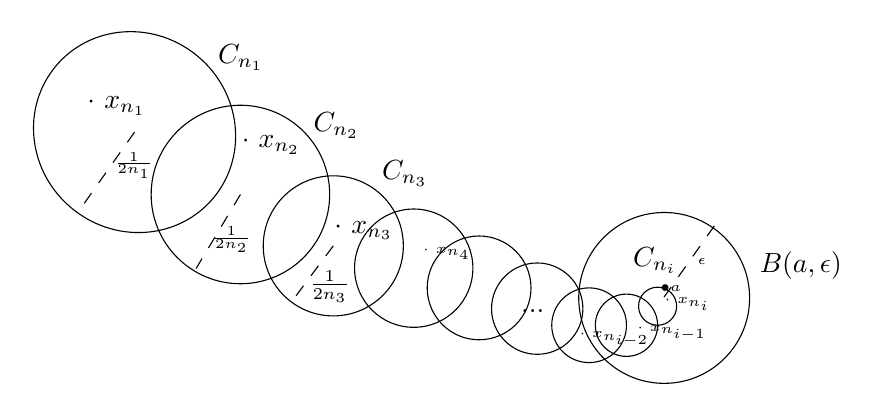
\begin{tikzpicture}[x=0.75pt,y=0.75pt,yscale=-1,xscale=1]
%uncomment if require: \path (0,300); %set diagram left start at 0, and has height of 300

%Shape: Circle [id:dp18973194445002073] 
\draw   (76.58,142.11) .. controls (73.77,115.44) and (93.16,92.4) .. (119.9,90.65) .. controls (146.64,88.9) and (170.6,109.11) .. (173.42,135.78) .. controls (176.24,162.45) and (156.84,185.49) .. (130.1,187.24) .. controls (103.36,188.98) and (79.4,168.78) .. (76.58,142.11) -- cycle ;
%Shape: Circle [id:dp43877875146716416] 
\draw   (187,193.75) .. controls (187,175.11) and (202.11,160) .. (220.75,160) .. controls (239.39,160) and (254.5,175.11) .. (254.5,193.75) .. controls (254.5,212.39) and (239.39,227.5) .. (220.75,227.5) .. controls (202.11,227.5) and (187,212.39) .. (187,193.75) -- cycle ;
%Shape: Circle [id:dp9005071318397828] 
\draw   (133,169) .. controls (133,145.25) and (152.25,126) .. (176,126) .. controls (199.75,126) and (219,145.25) .. (219,169) .. controls (219,192.75) and (199.75,212) .. (176,212) .. controls (152.25,212) and (133,192.75) .. (133,169) -- cycle ;
%Shape: Circle [id:dp13428568409862018] 
\draw   (231,204.5) .. controls (231,188.76) and (243.76,176) .. (259.5,176) .. controls (275.24,176) and (288,188.76) .. (288,204.5) .. controls (288,220.24) and (275.24,233) .. (259.5,233) .. controls (243.76,233) and (231,220.24) .. (231,204.5) -- cycle ;
%Shape: Circle [id:dp512751770725111] 
\draw   (266,214) .. controls (266,200.19) and (277.19,189) .. (291,189) .. controls (304.81,189) and (316,200.19) .. (316,214) .. controls (316,227.81) and (304.81,239) .. (291,239) .. controls (277.19,239) and (266,227.81) .. (266,214) -- cycle ;
%Shape: Circle [id:dp49620252416122534] 
\draw   (297,224) .. controls (297,211.85) and (306.85,202) .. (319,202) .. controls (331.15,202) and (341,211.85) .. (341,224) .. controls (341,236.15) and (331.15,246) .. (319,246) .. controls (306.85,246) and (297,236.15) .. (297,224) -- cycle ;
%Shape: Circle [id:dp6328081171133146] 
\draw   (326,232) .. controls (326,222.06) and (334.06,214) .. (344,214) .. controls (353.94,214) and (362,222.06) .. (362,232) .. controls (362,241.94) and (353.94,250) .. (344,250) .. controls (334.06,250) and (326,241.94) .. (326,232) -- cycle ;
%Shape: Circle [id:dp3553720531580573] 
\draw   (347,232) .. controls (347,223.72) and (353.72,217) .. (362,217) .. controls (370.28,217) and (377,223.72) .. (377,232) .. controls (377,240.28) and (370.28,247) .. (362,247) .. controls (353.72,247) and (347,240.28) .. (347,232) -- cycle ;
%Shape: Circle [id:dp7091481831610205] 
\draw   (367.83,222.83) .. controls (367.83,217.77) and (371.94,213.67) .. (377,213.67) .. controls (382.06,213.67) and (386.17,217.77) .. (386.17,222.83) .. controls (386.17,227.9) and (382.06,232) .. (377,232) .. controls (371.94,232) and (367.83,227.9) .. (367.83,222.83) -- cycle ;
%Shape: Circle [id:dp8694211134780476] 
\draw   (339,218.83) .. controls (339,196.1) and (357.43,177.67) .. (380.17,177.67) .. controls (402.9,177.67) and (421.33,196.1) .. (421.33,218.83) .. controls (421.33,241.57) and (402.9,260) .. (380.17,260) .. controls (357.43,260) and (339,241.57) .. (339,218.83) -- cycle ;
%Straight Lines [id:da06861963058135157] 
\draw  [dash pattern={on 4.5pt off 4.5pt}]  (125,138.94) -- (97.67,177.67) ;
%Straight Lines [id:da06667534021798405] 
\draw  [dash pattern={on 4.5pt off 4.5pt}]  (176,169) -- (154.67,204.67) ;
%Straight Lines [id:da4312694360461673] 
\draw  [dash pattern={on 4.5pt off 4.5pt}]  (220.75,193.75) -- (200.67,220.67) ;
%Straight Lines [id:da8658836143554338] 
\draw  [dash pattern={on 4.5pt off 4.5pt}]  (404.34,184.11) -- (377,222.83) ;

% Text Node
\draw (101,120.4) node [anchor=north west][inner sep=0.75pt]    {$\cdot \ x_{n_{1}}$};
% Text Node
\draw (175.42,139.18) node [anchor=north west][inner sep=0.75pt]    {$\cdot \ x_{n_{2}}$};
% Text Node
\draw (220,180.4) node [anchor=north west][inner sep=0.75pt]    {$\cdot \ x_{n_{3}}$};
% Text Node
\draw (262.56,192.86) node [anchor=north west][inner sep=0.75pt]  [font=\tiny,rotate=-358.91]  {$\cdot \ x_{n_{4}}$};
% Text Node
\draw (310,223.4) node [anchor=north west][inner sep=0.75pt]    {$...$};
% Text Node
\draw (338,233.4) node [anchor=north west][inner sep=0.75pt]  [font=\tiny]  {$\cdot \ x_{n_{i-2}}$};
% Text Node
\draw (365.83,230.23) node [anchor=north west][inner sep=0.75pt]  [font=\tiny]  {$\cdot \ x_{n_{i-1}}$};
% Text Node
\draw (379,217.07) node [anchor=north west][inner sep=0.75pt]  [font=\tiny]  {$\cdot \ x_{n_{i}}$};
% Text Node
\draw (377,211.4) node [anchor=north west][inner sep=0.75pt]  [font=\tiny]  {$\bullet a$};
% Text Node
\draw (164,95.4) node [anchor=north west][inner sep=0.75pt]    {$C_{n_{1}}$};
% Text Node
\draw (210,128.4) node [anchor=north west][inner sep=0.75pt]    {$C_{n_{2}}$};
% Text Node
\draw (243,151.4) node [anchor=north west][inner sep=0.75pt]    {$C_{n_{3}}$};
% Text Node
\draw (364,193.4) node [anchor=north west][inner sep=0.75pt]    {$C_{n_{i}}$};
% Text Node
\draw (425,195.4) node [anchor=north west][inner sep=0.75pt]    {$B( a,\epsilon )$};
% Text Node
\draw (395,198.4) node [anchor=north west][inner sep=0.75pt]  [font=\tiny]  {$\epsilon $};
% Text Node
\draw (114,147.4) node [anchor=north west][inner sep=0.75pt]  [font=\tiny]  {$\frac{1}{2n_{1}}$};
% Text Node
\draw (161,183.4) node [anchor=north west][inner sep=0.75pt]  [font=\fontsize{0.38em}{0.46em}\selectfont]  {$\frac{1}{2n_{2}}$};
% Text Node
\draw (208,204.4) node [anchor=north west][inner sep=0.75pt]  [font=\footnotesize]  {$\frac{1}{2n_{3}}$};
\end{tikzpicture}\\
%%%%%%%%%%%%%%%%%%%%%%%%%%%%%%%%%%%%%%%%%%%%%%%%%%%%%%%%%%%
But this means that $C_{n_i} \subset B(a,\epsilon)\subset S$, contrary to hypothesis.\\
\textit{Step 2: Show that if $X$ is sequentially compact, then for any $\epsilon > 0$, $\exists$ a finite covering of $X$ by open $\epsilon$-balls.}\\
Suppose $\ex\epsilon > 0$ such that $X$ cannot be covered by finitely many $\epsilon$-balls, then pick any point $x_1\in X$, $B(x_1,\epsilon)\subsetneq X$ otherwise $X$ could be covered by a single $\epsilon$-ball. Now choose $x_2\notin B(x_1,\epsilon)$. Inductively, choose 
$$
    x_{n+1}\notin B(x_1,\epsilon)\cup\dots\cup B(x_n,\epsilon)
$$
since these balls do not cover $X$. Note that by construction $d(x_{n+1},x_i)\geq\epsilon $ for $i = 1,\dots, n$. Therefore, the sequence $(x_n)$ can have no convergent subsequence. In particular, $X$ is not sequentially compact.\\
\textit{Step 3: Show that if $X$ is sequentially compact, then $X$ is compact.}\\
Let $A$ be an open covering of $X$. Because $X$ is sequentially compact, the open covering $A$ has a Lebesgue number $\delta$ by step 1. Let $\epsilon=\frac{\delta}{3}$. By step 2, we can use sequential compactness of $X$ to find a finite covering of $X$ by open $\epsilon$-balls. Each of these balls has diameter at most $2\cdot\frac{\delta}{3}$, so it lies in an element of $A$. Choosing one such element of $A$ for each of these finitely many $\epsilon$-balls, we obtain a finite subcollection of $A$ that covers $X$.
\end{proof}
\begin{lemma}
    Additionally, assume Y is Hausdorff and f is injective...
\end{lemma}
\section{Tikhonov's Revolutionary Result}
\begin{definition}
    order of sets, an order (=a partial order order) on a set $S$ is a linearly relation $\leq$.
\end{definition}
\begin{definition}[F.I.P.]
    A collection of subsets $\{C_a\}$ of a set $X$ has the finite intersection property(F.I.P.) if any finite intersection of this collection is not empty. More precisely, for any finite subcollection $\{C_{a_1},\dots,C_{a_n}\}\subseteq \{C_a\}$, $C_{a_1}\cap\dots\cap C_{a_n}\neq\emptyset$.
\end{definition}
\begin{theorem}[Tikhonov Part I]
    Let $X$ be a set, $A$ be a collection of subsets of $X$ having the FIP. Then there is a collection $D$ of subsets of $X$ such that $D$ contains $A$, and $D$ has the FIP, and no collection of subsets of $X$ that properly contains $D$ has FIP. Putting this into human language: $\ex$ a maximal collection of subsets with the FIP property.
\end{theorem}
\begin{proof}
    By hypothesis, we have a collection $A$ of subsets of $X$ that has the FIP. Let 
    $$
        B=\{S_i\subseteq X|S_1\cap\dots\cap S_n\neq\emptyset\}\qquad\mb A=\{B|A\subset B\}
    $$ 
    We use proper inclusion $\subsetneq$ as our strict partial order on $\mb A$. We need to show that $\mb A$ has a maximal element $D$. To apply Zorn’s lemma, we must show that if $\mb B \subseteq\mb A$ that is simply ordered by proper inclusion, then $\mb B$ has an upper bound in $\mb A$. We shall show in fact that the collection
    $$
        C=\bigcup_{B\in\mb B}B=\bigcup\{S_i\subseteq X|S_1\cap\dots\cap S_n\neq\emptyset\}
    $$
    is an element of $\mb A$; then it is the required upper bound on $\mb B$. Now we have two things to check (I) $A\subset C$: by definition, each element of $\mb B\subseteq \mb A$ contains $A$. (II) $C$ satisfies the FIP: let $S_1,\dots, S_n$ be elements of $C$. Because $C$ is the union of the elements of $\mb B$, for each i we have $S_i\in B_i\in\mb B$. The superset $\{B_1,\dots,B_n\}\subseteq\mb B$, so it is simply ordered by the relation of proper inclusion. Being finite, it has a largest element; that is, there is an index $k$ such that $B_i\subset B_k$ for $1\leq i\leq n$. Then all the sets $S_1,\dots,S_n$ are elements of $B_k$. Since $B_k$ has the FIP, the intersection of the sets $S_1,\dots,S_n$ is nonempty.
\end{proof}
\begin{theorem}[Tikhonov Part II]
    Let X be a set; let $M$ be a collection of subsets of $X$ that is maximal with respect to the FIP. Then:
    \begin{enumerate}
        \item[(a)] Any finite intersection of elements of $M$ is an element of $M$.
        \item[(b)] If $A$ is a subset of $X$ that intersects every element of $M$, then $A$ is an element of $M$.
    \end{enumerate}
\end{theorem}
\begin{proof} We may use (a) for the proof of (b).\\
    (a) Let $B$ equal the intersection of finitely many elements of $M$. Define a collection $E=M \cup \{B\}$. We show that $E$ has the finite intersection property; then maximality of $M$ implies that $B\in E = M$ as desired.
    Take finitely many elements of $E$. If none of them is the set $B$, then their intersection is nonempty because $M$ has the FIP. If one of them is the set $B$, then their intersection is of the form $D_1\cap\dots\cap D_m\cap B$, where $D_i\in M$. Since $B$ equals a finite intersection of elements of $M$, this set is nonempty.\\
    (b) Given $A$, define $E = M\cup \{ A\}$. We show that $E$ has the FIP, from which we conclude that $A$ belongs to $M$. Take finitely many elements of $E$. If none of them is the set $A$, their intersection is automatically nonempty. Otherwise, it is of the form $D_1\cap\dots\cap D_n\cap A$. Now $D_1\cap\dots\cap D_n$ belongs to $M$ by (a); therefore, this intersection is nonempty, by hypothesis.
\end{proof}
\begin{theorem}[Tikhonov Part III]
    An arbitrary product of compact spaces is compact in the product topology.
\end{theorem}
\begin{proof}
    Let each $X_a$ be compact, we have $X:=\prod_{a\in J}X_a$. Let $\mc A$ be a collection of subsets of $X$ having the FIP. We prove that the intersection $\bigcap_{A\in\mc A}\overline A\neq \emptyset$. Compactness of $X$ follows.

    Applying Part I, choose a collection $\mc D$ of subsets of $X$ such that $\mc A\subset\mc D$ and $\mc D$ is maximal with the FIP. Then we need to show $\bigcap_{D\in\mc D}\overline D\neq\emptyset$, which will imply $\bigcap_{A\in\mc A}\overline A\neq \emptyset$.

    Given $a\in J$, let $\pi_a: X\ra X_a$ be the projection map. The collection $\{\pi_a(D)|D\in\mc D\}$ has the FIP because $\mc D$ does. By compactness of $X_a$, we can for each $a$ choose a point $x_a\in X_a$ such that $x_a\in\bigcap_{D\in\mc D}\overline{\pi_a(D)}$. Let $x=(x_a)_{a\in J}\in\prod_{a\in J} X_a$. The set $U_b$ is a neighborhood of $x_b$ in $X_b$. Since $x_b\in \overline{\pi_b(D)}$ by definition, $U_b$ intersects $\pi_b(D)$ in some point $\pi_b(y)$ (recall the definition for closure), where $y\in D$. Then it follows that $y \in\pi\inv(U_b)\cap D$. It follows from (b) of Part II that every \textit{subbasis} element containing $x$ belongs to $\mc D$. And then it follows from (a) of Part II that every \textit{basis} element containing $x$ belongs to $\mc D$. Since $\mc D$ has the FIP, this means that every basis element containing $x$ intersects every element of $\mc D$; hence $x\in \overline{D}$ for every $D\in\mc D$ as desired.
\end{proof}
\section{SC Compactification}
\begin{definition}
    A \textbf{compactification} of a space $X$ is a compact Hausdorff space $Y$ containing $X$ as a subspace such that $\overline{X} = Y$. Two compactifications $Y_1$ and $Y_2$ of $X$ are said to be \textbf{equivalent} if there is a homeomorphism $h : Y_1\ra Y_2$ such that $h(x) = x$ for every $x\in X$.
\end{definition}
\begin{lemma}[SC helper]
    Let $X$ be a space; suppose that $h:X\ra Z$ is an imbedding of $X$ in the compact Hausdorff space $Z$. Then there exists a corresponding compactification $Y$ of $X$; it has the property that there is an imbedding $H : Y\ra Z$ that equals $h$ on $X$. The compactification $Y$ is uniquely determined up to equivalence.
\end{lemma}
\begin{proof}
    \textcolor{lightgray}{Given $h$, let $X_0=h(X)\subset Z$, and let $Y_0$ denote its closure in $Z$. Then $Y_0$ is a compact Hausdorff space and $\overline{X}_0 = Y_0$ (by the compactness of $Z$); therefore, $Y_0$ is a compactification of $X_0$.
    Now we show uniqueness. Recall that two compactifications $Y$ and $Y_0$ are equivalent if we may construct some homeomorphism $h : Y\ra Y_0$ such that $h(x) = x$ for every $x\in X$. To do this we begin by choosing a set $S$ where $S\cap X =\emptyset$ and where there is some map $k : S\ra Y_0\setminus X_0$ such that $k$ is a bijection. That is, $S$ acts as the boundary of $X_0$. Using the properties of this map we may define $Y = X\cup S$, with a new bijective map $H : Y\ra Y_0$ where
        \begin{center}
            $H(y)=
            \begin{cases}
                h(y)& \text{ for } y\in X\\
                k(y)& \text{ for } y\in S 
            \end{cases}$
        \end{center}
    We then give one more property to $Y$ to give it a topology. Suppose that $U$ is a subset of $Y$. Then $U$ may only be open in $Y$ iff $H(U)$ is open in $Y_0$. The mapping $H$ is a bijection and therefore a homeomorphism. It is also true that $H(y) = h(y)$ for all $y\in X$ and so we can extend the range of $H$ to get an appropriate imbedding $H: Y\ra Z$.
    Now suppose $Y_i$ is a compactification of $X$ and that $Hi : Y_i\ra Z$ is an imbedding that is an extension of $h$, for $i = 1, 2$. Now $H_i$ maps $X$ onto $h(X) = X_0$. 
    Because $H_i$ is continuous, it must map $Y_i$ into $\overline{X_0}$; because $H_i(Y_i)$ contains $X_0$ and is closed(being compact), it contains $\overline{X}_0$. 
    Hence $H_i(Y_i) = \overline{X}_0$, and $H\inv\circ H_1$ defines a homeomorphism of $Y_1$ with $Y_2$ that equals the identity on $X$.}
    \end{proof}
\begin{definition}[SC-Comp]
    The SC compactification of $X$ is a compact Hausdorff space $\beta(X)$ containing $X$ as a subspace, such that $\overline{X}=\beta(X)$ and for any bounded continuous function $f:X\ra\R$, $\ex$ a bounded continuous extension $f':\beta(X)\ra\R$.
\end{definition}
\begin{definition}[CRegular]
    $X$ is completely regular if each one-point subset of $X$ is closed and for any $x\in X$ and any closed set $C\subseteq X$, if $x\notin C$, then $\ex$ a continuous function $f:X\ra [0,1]$ such that $f(c)=0$ for all $c\in C$ and $f(x)=1$.
\end{definition}
\begin{theorem}[Existance of SC-Comp]
    Let $X$ be a completely regular space, there exist a compactification $Y$ of $X$ with the property that every bounded continuous map $f: X\ra\R$ extends uniquely to a continuous map $Y$ into $\R$.
\end{theorem}
\begin{proof}
    Let $\{f_a\}_{a\in J}$ be the set of all bounded real functions. Define real intervals $I_a$ to contain $f_a(X)$: $I_a=[\inf(f_a(X)),\sup(f_a(X))]$. These intervals are compact, thus by Tikhnov $\prod_{a\in J}I_a$ is also compact. Define 
    $$
        h:X \ra \prod_{a\in J}I_a\qquad h(x)=(f_a(x))_{a\in J}
    $$
    Now, we know from the SC helper that for any imbedding $h$ of a completely regular space $X$ into a compact Hausdorff space $\prod I_a$ has a corresponding compactification $Y$. Then there is a mapping $H$ of the compactification of $X$ induced by $h$ that satisfies the SC helper
    $$
        H: Y\ra \prod I_a
    $$
    Let $f$ be any bounded continuous real function, $f\in\{f_a\}_{a\in J}$. We will show $f$ can be extended to $Y$. Since $f\in\{f_a\}_{a\in J}$, $\ex b$ such that $f=f_b$. Define $\phi_b: \prod I_a\ra I_b$, now compose it with our imbedding $H$
    $$
        \phi_b\circ H: Y\ra \R^J\ra \R
    $$
    This is continuous. Since $H|_X=h$
    $$
        \phi_b(H(x))=\phi(h(x))=\phi(f_a(x))_{a\in J}=f_b(x)
    $$
    Thus, we are able to construct an appropriate extension for any real valued function that is bounded and continuous over $X$.
\end{proof}
\begin{theorem}[Uniqueness of SC-Comp]
    Let $A\subset X$; let $f: A\ra Z$ be a continuous map of $A$ into the Hausdorff space $Z$. There is at most one extension of $f$ to a continuous function $g : \overline{A}\ra Z$.
\end{theorem}
\begin{proof}
\textcolor{lightgray}{
    Suppose that $g, g' : \overline{A}\ra X$ are two different extensions of $f$; choose $x$ so that $g(x)\neq g'(x)$. Let $U$ and $U'$ be disjoint neighborhoods of $g(x)$ and $g'(x)$, respectively. Choose a neighborhood $V$ of $x$ so that $g(V)\subset U$ and $g'(V)\subset U'$. Now $V$ intersects $A$ in some point $y$; then $g(y)\in U$ and $g'(y)\in U'$. But since $y\in A$, we have $g(y)= f(y)$ and $g'(y) = f (y)$. This contradicts the fact that $U$ and $U'$ are disjoint.
    }
\end{proof}
\section{Complete Metric Space}
\begin{definition}
    Cauchy sequence.
\end{definition}
\begin{definition}
    A metric space is complete if any Cauchy sequence in $X$ converges in $X$.
\end{definition}
\begin{lemma}
    Let $(x_i)$ be a Cauchy sequence in $(X,d)$. Then TFAE
    \begin{enumerate}
        \item $(x_i)$ converges in $X$.
        \item There is a converging subsequence of $(x_i)$ in $X$.
    \end{enumerate}
\end{lemma}
\begin{proof}
    (1)$\Ra$(2): take the subsequence to be itself. (2)$\Ra$(1): Let $(x_{n_i})$ be a subsequence converging to some $x\in X$. Take any $\epsilon>0$, since $(x_n)$ is Cauchy, $\exists N\in \mathbb{N}$ such that $\forall m,n\geq N$, $d(x_m,x_n)<\epsilon/2$. Since $x_{n_i}\ra x, i\ra \infty$, $\exists$ an index $i\in\mathbb{N}$ such that $n_{i}>N$ and $d(x_{n_i},x)<\epsilon/2$. Take $m=n_i$, then $d(x_n,x)\leq d(x_n,x_{n_i})+d(x_{n_i},x)<\epsilon/2+\epsilon/2=\epsilon\Ra x_n\ra x$.
\end{proof}
\begin{theorem}
    Every compact metric space is complete. 
\end{theorem}
\begin{proof}
    Note that in metric spaces the notions of compactness and sequential compactness coincide. Let $x_n$ be a Cauchy sequence in the metric space $X$. Since $X$ is sequentially compact there is a convergent subsequence $x_{n_k}\to x \in X$. 
    
    All that now remains to be shown is that $x_n \to x$. Since $x_{n_k}\to x$ there is $N_1$ with $n_k \ge N_1$ implies $d(x_{n_k},x)<{\varepsilon\over 2}$. Let $N_2$ be such that $n,m\ge N_2$ implies $d(x_n,x_m)<{\varepsilon \over 2}$. 
    Let $n\geq N=\max(N_1,N_2)$ and pick some $n_k\geq N$. Then
    $$ d(x_n,x)\le d(x_n,x_{n_k})+d(x_{n_k},x)<\varepsilon.$$
    Hence $X$ is complete. 
\end{proof}
\begin{lemma}
    Every Cauchy sequence is bounded.
\end{lemma}
\begin{proof}
    Let $(a_{n})$ be Cauchy. We choose $ 0<\epsilon_{0}$. So $ \forall \; n>m\geq N_{0}$ we have that $\vert a_{n}-a_{m} \vert < \epsilon_{0}$. Therefore $(a_{n})$ is bounded for all $ m \geq N_{0} $ by $ \epsilon_{0} $. Since $ \mathbb{N}_{N_{0}}$ is finite, it is bounded. So, for all $ m<N_{0} $, $ (a_{n})$ is bounded. Therefore $(a_{n})$ is bounded.
\end{proof}
\begin{theorem}
    $\R^n$ is complete for each $n\in \N$ (w.r.t. any metric $d_p$ for any $p\in[1,\infty]$)
\end{theorem}
\begin{proof}
    Take any Cauchy sequence $(x_n)$ in $\R^n$, it is bounded. $\Ra\{x_n|n\in \N\}$ is contained in some closed ball (w.r.t.$d_p$). This ball is closed in $\R^n$ and bounded $\Ra$ compact $\Ra$ sequentially compact $\Ra$ $\exists$ a subsequence of $(x_n)$ converging to some $x\in$ball $\Ra(x_n)$ converges to $x\in$ball$\subseteq\R^n$.
\end{proof}
\begin{definition}[Bounded Metric and Uniform Metric]
    $\overline d(x,y)=\MIN\{d(x,y),1\}$ is the \textbf{bounded metric}. Set $\vec{x}=\{x_{\alpha}\}_{\alpha\in J}$ and $\vec{y}=\{y_{\alpha}\}_{\alpha\in J}$. $\vec{x}$ and $\vec{y}$ are points of the Cartesian product $Y^J$. Define the \textbf{uniform metric} as $\overline{\rho}(\vec{x},\vec{y})=\sup\{\overline{d}(x_{\alpha},y_{\alpha})|\alpha\in J\}$. When viewing $Y^J$ as functions from $J$ to $Y$, we can define uniform metric corresponding to the metric $\overline{d}$ on $Y$ as $f,g: J\ra Y$, $\overline{\rho}=\sup\{\overline{d}(f(\alpha),g(\alpha))| \alpha\in J\}$. We can check $\overline{\rho}$ is indeed a metric.
\end{definition}
\begin{definition}
    Define for $x\in X$, $U\subseteq Y$ open: $S(x,U)=\{f: X\ra Y|f(x)=U\}\subseteq Y^X$.
\end{definition}
\begin{comment}
$S(x_1,U_1)\cap S(x_2,U_2)$, $\mc S=\{S(x,U)|x\in X, U\subseteq Y\}$ is a subbasis. If $X$ is finite, this will be a basis.
\end{comment}
\begin{theorem}
    If the space $Y$ is complete in the metric $d$, then the space $Y^J$ is complete in the uniform metric $\overline{\rho}$ corresponding to $d$.
\end{theorem}
\begin{proof}
    Observe that $\overline{d}(x,y)\leq d(x,y)$, then let $\{y_i\}$ be a sequence in $Y$. By the inequality, $\{y_i\}$ is Cauchy w.r.t. $d$ $\Ra$ $\{y_i\}$ is Cauchy w.r.t. $\overline{d}$. Also, $\{y_i\}$ converges in $Y$ w.r.t. $d$. $\Ra$ $\{y_i\}$ converges in $Y$ w.r.t. $\overline{d}$. It follows that if $(Y, d)$ is complete then $(Y, \overline{d})$ is complete. Let $\{f_i\}$ be a Cauchy sequence in $Y^J$ relative to $\overline{\rho}$. If we think of $\{f_i\}$ as functions, then the difference at a single point is less or equal to the supremum of all differences, hence we have the following inequality
    $$
        \overline{d}(f_n(\alpha),f_m(\alpha))\leq\overline{\rho}(f_n,f_m)
    $$
    for all $m,n$. This shows $\{f_{i}(\alpha)\}$ is Cauchy relative to $\overline{d}$. Then $\{f_i(\alpha)\}\ra y_{\alpha}$ to some $y_{\alpha}\in Y$. Let $f\in Y^J$ such that $f(\alpha)=y_{\alpha}$. Given $\epsilon > 0$, first choose $N$ large enough that $\overline{\rho}(f_n, f_m) < \epsilon/2$ whenever $n, m\geq N$. Then $\overline{d}(f_n(\alpha),f_m(\alpha))<\epsilon/2$. Since $\{f_i\}\ra f$ at $\alpha$, if we let $m$ large, $\overline{d}(f_n(\alpha),f(\alpha))\leq\epsilon/2$. Let $f$ be the function that does this for all $\alpha$ when $n\geq N$, we have 
    $$
        \overline{\rho}(f_n,f)\leq\epsilon/2<\epsilon
    $$
    This proves that $\{f_n\}\ra f$ as required.
\end{proof}
\begin{definition}[Set of Continuous/Bounded Function]
    A function $f$ is said to be \textbf{bounded} if its image $f(X)$ is a bounded subset of the metric space $(Y, d)$. $C(X,Y)$ and $B(X,Y)$ are the set of continuous and the set of bounded functions respectively.
\end{definition}
\begin{theorem}
    Let $X$ be a topological space and let $(Y, d)$ be a metric space. The set $C(X, Y )$ of continuous functions is closed in $Y^X$ under the uniform metric. So is the set $B(X, Y )$ of bounded functions. Therefore, if Y is complete, these spaces are complete in the uniform metric.
\end{theorem}
\begin{proof}
    We recall the uniform limit theorem to prove a part of the theorem.\\
    Part 1: if the sequence $\{f_n\}\subset Y^X$ converges to some element $f\in Y^X$ relative to $\overline{\rho}$, then for any $\epsilon>0$, choose some $N$ such that $\overline{\rho}(f_n,f) <\epsilon$, $\forall n>N$. Since $\overline{d}$ is bounded by $\overline{\rho}$. we have 
    $$
        \overline{d}(f_n(x).f(x))\leq\overline{\rho}(f_n,f)<\epsilon \Ra \{f_n\}\ra f
    $$
    Part 2: let $f\in Y^X$ be any limit point of $C(X,Y)$. Then there is a sequence $\{f_n\}\subset C(X,Y)$ such that $\{f_n\}\ra f$ relative to $\overline{\rho}$. By the uniform limit theorem, the limit should also be a continuous function, thus $f\in C(X,Y)$. Then $C(X,Y)$ contains all limit points. It is closed.\\
    Part 3: let $f\in Y^X$ be any limit point of $B(X,Y)$. Then there is a sequence $\{f_n\}\subset B(X,Y)$ such that $\{f_n\}\ra f$. 
    Since convergence, $\exists N$ such that $\overline{\rho}(f_N, f)<1/2$. 
    Then for $x\in X$, we have $\overline{d}( f_N (x), f (x)) < 1/2$, which implies that $d( f_N (x), f (x)) < 1/2$. It follows that if $M$ is the diameter of the set $f_N (X)$, then $f (X)$ has diameter at most $M + 1$.
    Hence $f\in B(X, Y )$.\\ 
    We conclude that $C(X, Y )$ and $B(X, Y )$ are complete in the metric $\overline{\rho}$ if $Y$ is complete in $d$.
\end{proof}
\begin{definition}[Sup Metric]
    If $(Y,d)$ is a metric space, one can define another metric on the set $B(X, Y )$ by the equation $\rho( f, g) = \sup\{d( f (x), g(x)) | x\in X\}$. It is easy to see that $\rho$ is well-defined(?), for the set $f (X)\cup g(X)$ is bounded if both $f (X)$ and $g(X)$ are. The metric $\rho$ is called the \textbf{sup metric}.
\end{definition}
\begin{remark}
    For $f,g\in B(X,Y)$, we have $\overline{\rho}( f, g) = \min\{\rho( f, g), 1\}$.
\end{remark}
\begin{theorem}
    Let $(X, d)$ be a metric space. There is an isometric imbedding of $X$ into a complete metric space.
\end{theorem}
\begin{proof}
    Let $B(X,\R)$ be the usual stuff. Let $x_0$ be a fixed point of $X$. Define
    $$
        \phi_a: X\ra \R,\qquad \phi_a(x)=d(x,a)-d(x,x_0)
    $$
    From triangle inequality we have $d(x, a)\leq d(x, b) + d(a, b)$ and $d(x, b)\leq d(x, a) + d(a, b)$. By subtraction, $|d(x,a) - d(x,b)|\leq d(a,b)$. Setting $b=x_0$ we showed $|\phi_a(x)|\leq |d(a,x_0)|$ for all $x$. $\phi_a(x)$ is bounded. Define
    $$
        \Phi: X\ra B(X,\R),\qquad \Phi(a)=\phi_a
    $$
    We show that $\Phi$ is an isometric imbedding of $(X,d)$ into the complete metric space $(B(X,\R),\rho)$. By definition,
    $$
        \rho(\phi_a,\phi_b)=\sup\{|\phi_a-\phi_b|\}=\sup\{|d(x,a)-d(x,b)|\}\leq \sup\{d(a,b)\}=d(a,b)
    $$
    Notice that the inequality $|d(x,a)-d(x,b)|\leq d(a,b)$ cannot be strict when $x=a$. Thus we have 
    $$
        \rho(\phi_a,\phi_b)=\sup\{|d(x,a)-d(x,b)|\}=\sup\{d(a,b)\}=d(a,b)
    $$
    which shows $\rho(\phi_a,\phi_b) = d(a,b)$ proving $\Phi$ is an isometric imbedding.
\end{proof}
\begin{definition}[Completion]
    Let $X$ be a metric space. If $h : X\ra Y$ is an isometric imbedding of $X$ into a complete metric space $Y$, then the subspace $h(X)$ of $Y$ is a complete metric space. It is called the \textbf{completion} of $X$.
\end{definition}
\begin{definition}[Pointwise Convergence]
    Given a point $x\in X$ and an open set $U \subset Y$ , let $S(x,U)=\{f | f \in Y^X\text{ and }f(x)\in U\}$. The sets $S(x,U)$ are a subbasis for topology on $Y^X$, which is called the topology of \textbf{pointwise convergence}.
\end{definition}
\begin{remark}
    The general basis element for this topology is a finite intersection of subbasis elements $S(x,U)$. Thus a typical basis element about the function $f$ consists of all functions $g$ that are "close" to $f$ at finitely many points. Intuitively
\begin{center}
\tikzset{every picture/.style={line width=0.75pt}} %set default line width to 0.75pt        

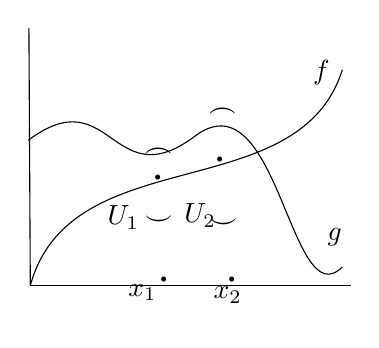
\begin{tikzpicture}[x=0.75pt,y=0.75pt,yscale=-1,xscale=1]
%uncomment if require: \path (0,300); %set diagram left start at 0, and has height of 300

%Straight Lines [id:da06657861788112385] 
\draw    (199.33,97) -- (200,221) ;
%Straight Lines [id:da18363761005445434] 
\draw    (200,221) -- (354.33,221) ;
%Curve Lines [id:da29208260806791775] 
\draw    (200,221) .. controls (219.33,150) and (329.33,184) .. (350.33,117) ;
%Curve Lines [id:da11748915891212541] 
\draw    (199,151) .. controls (239,121) and (239.33,179) .. (279.33,149) .. controls (319.33,119) and (325.33,237) .. (350.33,212) ;

% Text Node
\draw (268.79,151.93) node [anchor=north west][inner sep=0.75pt]  [font=\small,rotate=-89.51] [align=left] {( \ \ \ \ \ \ )};
% Text Node
\draw (257,163.4) node [anchor=north west][inner sep=0.75pt]  [font=\LARGE]  {$\cdot $};
% Text Node
\draw (299.79,132.93) node [anchor=north west][inner sep=0.75pt]  [font=\small,rotate=-89.51] [align=left] {( \ \ \ \ \ \ \ \ \ \ \ )};
% Text Node
\draw (287,154.4) node [anchor=north west][inner sep=0.75pt]  [font=\LARGE]  {$\cdot $};
% Text Node
\draw (236,181.4) node [anchor=north west][inner sep=0.75pt]    {$U_{1}$};
% Text Node
\draw (273,180.4) node [anchor=north west][inner sep=0.75pt]    {$U_{2}$};
% Text Node
\draw (260,212.4) node [anchor=north west][inner sep=0.75pt]  [font=\LARGE]  {$\cdot $};
% Text Node
\draw (293,212.4) node [anchor=north west][inner sep=0.75pt]  [font=\LARGE]  {$\cdot $};
% Text Node
\draw (246,219.4) node [anchor=north west][inner sep=0.75pt]    {$x_{1}$};
% Text Node
\draw (287,220.4) node [anchor=north west][inner sep=0.75pt]    {$x_{2}$};
% Text Node
\draw (335,111.4) node [anchor=north west][inner sep=0.75pt]    {$f$};
% Text Node
\draw (342,192.4) node [anchor=north west][inner sep=0.75pt]    {$g$};
\end{tikzpicture}
\end{center}
where $g\in S(x_1,U_1)\cap S(x_2,U_2)$.
\end{remark}
\begin{definition}[Compact Convergence]
    Let $(Y,d)$ be a metric space. Let $X$ be a topological space. Given an element $f\in Y^X$, a compact subspace $C\subset X$, and a number $\epsilon > 0$, let $B_C(f,\epsilon)$ denote the set of all those elements $g\in Y^X$ for which
    $$
        \sup\{d( f (x), g(x)) | x\in C\} < \epsilon
    $$
    The sets $B_C ( f, \epsilon)$ form a basis for a topology on $Y^X$. It is called the topology of \textbf{compact convergence}.
\end{definition}
\begin{lemma}
    Check that $\mc B_{cpt}=\{B_C(f,\epsilon)\}$ form a basis of $Y^X$.
\end{lemma}
\begin{proof}
    Check both criteria \circled{1} for any $h\in Y^X$, let $C$ be some compact set that $h$ passes through. Pick an appropriate $\epsilon>0$ we have $h\in B_C(h,\epsilon)$. \circled{2} let $f\in B_{C_1}(f_1,\epsilon_1)\cap B_{C_2}(f_2,\epsilon_2)$. We choose $C_3=C_1\cap C_2$, $f_3=f$, and $\epsilon_3= \min\{\epsilon_1,\epsilon_2\}$. We conclude that $\mc B_{cpt}$ is a basis and $\mc T_{cpt}$ is the topology generated by $\mc B_{cpt}$.
\end{proof}
\begin{definition}
    Define 
    $$
        B_X(f,\epsilon)=\{g:X\ra Y|\underset{x\in \textcolor{red}{X}}{\sup}\{d(f(x),g(x))\}<\epsilon\}
    $$
    for $f\in Y^X,\epsilon>0$ as basis elements. We get the basis for the \textbf{uniform convergence} topology $\mc B_{uni}=\{B_X(f,\epsilon)\}$. Comparing to basis elements of $\mc B_{cpt}$
    $$
        B_C(f,\epsilon)=\{g:X\ra Y|\underset{x\in \textcolor{red}{C}}{\sup}\{d(f(x),g(x))\}<\epsilon\}
    $$
    Instead of requiring it to stay close on all of $X$, $B_X$ only requires it to stay close in a compact subset. Thus $\mc T_{cpt} \subset\mc T_{uni}$. Meanwhile, $\bigcap_i S(x_i,U_i)$ only requires it to stay close near finitely many points hence $\mc T_{pt} \subset\mc T_{cpt}$.
\end{definition}
\begin{theorem}
    Let $X$ be a space, and let $(Y,d)$ be a metric space. For the function space $Y^X$, the following inclusions hold:
    $$
        \mc T_{pt} \subset\mc T_{cpt}\subset\mc T_{uni}
    $$
    If $X$ is compact, the last two coincide, and if $X$ is discrete, the first two coincide.
\end{theorem}
\begin{proof}
    Clear.
\end{proof}
\begin{definition}
    Let $X$ and $Y$ be topological spaces. If $C$ is a compact subspace of $X$ and $U$ is an open subset of $Y$, define
    $$
        S(C,U)=\{f | f \in C(X,Y)\text{ and } f(C)\subset U\}
    $$
    The sets $S(C,U)$ form a subbasis for a topology on $C(X,Y)$ that is called the \textbf{compact-open} topology. Comparing to the pointwise convergence topology
    $$
        S(x,U)=\{f | f \in Y^X\text{ and }f(x)\in U\}
    $$
    we see that the compact-open topology is finer.
\end{definition}
\begin{theorem}
    Let $X$ be a space and let $(Y, d)$ be a metric space. On the set $C(X, Y )$, the compact-open topology and the topology of compact convergence coincide.
\end{theorem}
\begin{lemma}
    If $K$ is compact subset of $Y$ and $V$ is an open subset of $Y$ such that $K\subset V$. Then there exist an $\epsilon>0$ such that $U(K,\epsilon) \subset V$.
\end{lemma}
\begin{proof}[proof of the lemma]
    Consider the function $f:K\to\mathbb{R}$ defined by $f(x)=d(a,Y-V)$. Since the domain $K$ is compact, by the extreme value theorem, there is some point $x\in K$ at which the function $f$ attains its minimum value $\varepsilon$. 
    In a metric space, for every point $x$ and subset $A$, it can be easily proven that 
    $$
        d(x,A)=0\iff x\in\bar{A}.
    $$
    Note that $V$ is an open set, so its complement $Y-V$ is a closed set and hence $\overline{Y-V}=Y-V$. As we can see, we have $K\subseteq V$; that is, $K\cap(Y-V)=\emptyset$, so $f(x)>0$ for all $x\in K$. That is why $\varepsilon>0$. Then we need to show that $U(K,\varepsilon)\subseteq V$.\\
    We can prove it by contradiction. Suppose $y\in U(K,\varepsilon)$ but $y\notin V$. Then for every $x\in K$, we have 
    $$
        d(x,y)\geq d(x,Y-V)\geq\varepsilon.
    $$
    That is, 
    $$
        d(y,K)=\inf_{x\in K}{d(y,x)}\geq\varepsilon,
    $$
    producing a contradiction. 
\end{proof}
\begin{proof}[Proof of the theorem]
    If $A$ is a subset of $Y$ and $\epsilon > 0$, let $U(A,\epsilon)$ be the $\epsilon$-neighborhood of $A$. If $A$ is compact and $V$ is an open set containing $A$, then there is an $\epsilon > 0$ such that $U(A,\epsilon)\subset V$. Indeed, the minimum value of the function $d(a, X\setminus V)$ is the required $\epsilon$. (This is proven as the above lemma)
    
    We first prove that the topology of compact convergence is finer than the compact-open topology. Let $S(C,U)$ be a subbasis element for the compact-open topology, and let $f\in S(C,U)$. Because $f$ is continuous, $f(C)$ is a compact subset of the open set $U$. Therefore by the above, we can choose $\epsilon$ so that $\epsilon$-neighborhood of $f (C)\subset U$. Then $B_C(f,\epsilon)\subset S(C,U)$ as desired.

    Now we prove that the compact-open topology is finer than the topology of compact convergence. Let $f\in C(X,Y)$. Given an open set about $f$ in the topology of compact convergence, it contains a basis element of the form $B_C ( f,\epsilon)$. We shall find a basis element for the compact-open topology that contains $f$ and lies in $B_C ( f, \epsilon)$.

    Each point $x\in X$ has a neighborhood $V_x$ such that $f (\overline{V_x})$ lies in an open set $U_x$ of $Y$ having diameter less than $\epsilon$.
    [For example, choose $V_x$ so that $f(V_x)$ lies in the $\epsilon/4$-neighborhood of f (x). Then $f (\overline{V_x})$ lies in the $\epsilon/3$-neighborhood of $f (x)$, which has diameter at most $2\epsilon/3$.] Cover $C$ by finitely many such sets $V_x$, say for $x=x_1,\hdots,x_n$. Let $C =\overline{V_x}\cap C$. Then $C$ is compact, and the basis element
    $$
        S(C_{x_1} ,U_{x_1} )\cap\hdots\cap S(C_{x_n} ,U_{x_n} )
    $$
    contains $f$ and lies in $B_C ( f, \epsilon)$, as desired.
\end{proof}
\section{Some Arzela Shit}
Two versions of arzela thm: $X$ a topological space, $A\subseteq X$, $A$ is relatively compact if $\overline{A}$ in $X$ is compact. In other words, the shortest path problem: the shortest path may not exist. But this arzela thm allows us to take limits (inf of all paths). Formal statement
\begin{definition}
    Let $X$ be a top space, $(Y,d)$ be a metric space $C(X,Y)$. Let $F\subseteq C(X,Y)$ be a family of continuous functions $X\ra Y$. $F$ is \textbf{equicontinuous} if $\forall x_0\in X$, $\forall\epsilon>0$ $\exists$nbd $U$ of $x_0$ (in $X$) [s.t. forall $f\in F$, $f(U)\subseteq B(f(x_0),\epsilon)$] or [s.t. forall $f\in F$, forall $x\in U$ $d(f(x_0),f(x))<\epsilon$]
\end{definition}
\begin{example}
    see pic for 11/27.
\end{example}
\begin{theorem}[Arzela 1]
    Let $X$ be a topological space, $(Y,d)$ be a metric space and $F\subseteq C(X,Y)$. Put the compact convergence topology on $C(X,Y)$. If $F$ is pointwise relatively compact and equicontinuous, then $F$ is relatively compact in $C(X,Y)$.
\end{theorem}
\begin{theorem}[Arzela 2]
    Let $X$ be a topological space, $(Y,d)$ be a metric space. Put the compact convergence topology on $C(X,Y)$. Additionally, we assume that $X$ is Hausdorff and $\sigma$-compact(there is a sequence of compact sets in the space whose the union is the whole space, this is used to prove 1-countability). If $\{f_n\}\subseteq C(X,Y)$ is a sequence that is pointwise relatively compact and equicontinuous, then $\ex$ a subsequence of $\{f_n\}'$ that converges in $C(X,Y)$.
\end{theorem}
\bigskip
\end{document}
